% Options for packages loaded elsewhere
% Options for packages loaded elsewhere
\PassOptionsToPackage{unicode}{hyperref}
\PassOptionsToPackage{hyphens}{url}
%
\documentclass[
  a4paper,
]{book}
\usepackage{xcolor}
\usepackage{amsmath,amssymb}
\setcounter{secnumdepth}{5}
\usepackage{iftex}
\ifPDFTeX
  \usepackage[T1]{fontenc}
  \usepackage[utf8]{inputenc}
  \usepackage{textcomp} % provide euro and other symbols
\else % if luatex or xetex
  \usepackage{unicode-math} % this also loads fontspec
  \defaultfontfeatures{Scale=MatchLowercase}
  \defaultfontfeatures[\rmfamily]{Ligatures=TeX,Scale=1}
\fi
\usepackage{lmodern}
\ifPDFTeX\else
  % xetex/luatex font selection
\fi
% Use upquote if available, for straight quotes in verbatim environments
\IfFileExists{upquote.sty}{\usepackage{upquote}}{}
\IfFileExists{microtype.sty}{% use microtype if available
  \usepackage[]{microtype}
  \UseMicrotypeSet[protrusion]{basicmath} % disable protrusion for tt fonts
}{}
\makeatletter
\@ifundefined{KOMAClassName}{% if non-KOMA class
  \IfFileExists{parskip.sty}{%
    \usepackage{parskip}
  }{% else
    \setlength{\parindent}{0pt}
    \setlength{\parskip}{6pt plus 2pt minus 1pt}}
}{% if KOMA class
  \KOMAoptions{parskip=half}}
\makeatother
% Make \paragraph and \subparagraph free-standing
\makeatletter
\ifx\paragraph\undefined\else
  \let\oldparagraph\paragraph
  \renewcommand{\paragraph}{
    \@ifstar
      \xxxParagraphStar
      \xxxParagraphNoStar
  }
  \newcommand{\xxxParagraphStar}[1]{\oldparagraph*{#1}\mbox{}}
  \newcommand{\xxxParagraphNoStar}[1]{\oldparagraph{#1}\mbox{}}
\fi
\ifx\subparagraph\undefined\else
  \let\oldsubparagraph\subparagraph
  \renewcommand{\subparagraph}{
    \@ifstar
      \xxxSubParagraphStar
      \xxxSubParagraphNoStar
  }
  \newcommand{\xxxSubParagraphStar}[1]{\oldsubparagraph*{#1}\mbox{}}
  \newcommand{\xxxSubParagraphNoStar}[1]{\oldsubparagraph{#1}\mbox{}}
\fi
\makeatother


\usepackage{longtable,booktabs,array}
\usepackage{calc} % for calculating minipage widths
% Correct order of tables after \paragraph or \subparagraph
\usepackage{etoolbox}
\makeatletter
\patchcmd\longtable{\par}{\if@noskipsec\mbox{}\fi\par}{}{}
\makeatother
% Allow footnotes in longtable head/foot
\IfFileExists{footnotehyper.sty}{\usepackage{footnotehyper}}{\usepackage{footnote}}
\makesavenoteenv{longtable}
\usepackage{graphicx}
\makeatletter
\newsavebox\pandoc@box
\newcommand*\pandocbounded[1]{% scales image to fit in text height/width
  \sbox\pandoc@box{#1}%
  \Gscale@div\@tempa{\textheight}{\dimexpr\ht\pandoc@box+\dp\pandoc@box\relax}%
  \Gscale@div\@tempb{\linewidth}{\wd\pandoc@box}%
  \ifdim\@tempb\p@<\@tempa\p@\let\@tempa\@tempb\fi% select the smaller of both
  \ifdim\@tempa\p@<\p@\scalebox{\@tempa}{\usebox\pandoc@box}%
  \else\usebox{\pandoc@box}%
  \fi%
}
% Set default figure placement to htbp
\def\fps@figure{htbp}
\makeatother


% definitions for citeproc citations
\NewDocumentCommand\citeproctext{}{}
\NewDocumentCommand\citeproc{mm}{%
  \begingroup\def\citeproctext{#2}\cite{#1}\endgroup}
\makeatletter
 % allow citations to break across lines
 \let\@cite@ofmt\@firstofone
 % avoid brackets around text for \cite:
 \def\@biblabel#1{}
 \def\@cite#1#2{{#1\if@tempswa , #2\fi}}
\makeatother
\newlength{\cslhangindent}
\setlength{\cslhangindent}{1.5em}
\newlength{\csllabelwidth}
\setlength{\csllabelwidth}{3em}
\newenvironment{CSLReferences}[2] % #1 hanging-indent, #2 entry-spacing
 {\begin{list}{}{%
  \setlength{\itemindent}{0pt}
  \setlength{\leftmargin}{0pt}
  \setlength{\parsep}{0pt}
  % turn on hanging indent if param 1 is 1
  \ifodd #1
   \setlength{\leftmargin}{\cslhangindent}
   \setlength{\itemindent}{-1\cslhangindent}
  \fi
  % set entry spacing
  \setlength{\itemsep}{#2\baselineskip}}}
 {\end{list}}
\usepackage{calc}
\newcommand{\CSLBlock}[1]{\hfill\break\parbox[t]{\linewidth}{\strut\ignorespaces#1\strut}}
\newcommand{\CSLLeftMargin}[1]{\parbox[t]{\csllabelwidth}{\strut#1\strut}}
\newcommand{\CSLRightInline}[1]{\parbox[t]{\linewidth - \csllabelwidth}{\strut#1\strut}}
\newcommand{\CSLIndent}[1]{\hspace{\cslhangindent}#1}



\setlength{\emergencystretch}{3em} % prevent overfull lines

\providecommand{\tightlist}{%
  \setlength{\itemsep}{0pt}\setlength{\parskip}{0pt}}



 


\makeatletter
\@ifpackageloaded{tcolorbox}{}{\usepackage[skins,breakable]{tcolorbox}}
\@ifpackageloaded{fontawesome5}{}{\usepackage{fontawesome5}}
\definecolor{quarto-callout-color}{HTML}{909090}
\definecolor{quarto-callout-note-color}{HTML}{0758E5}
\definecolor{quarto-callout-important-color}{HTML}{CC1914}
\definecolor{quarto-callout-warning-color}{HTML}{EB9113}
\definecolor{quarto-callout-tip-color}{HTML}{00A047}
\definecolor{quarto-callout-caution-color}{HTML}{FC5300}
\definecolor{quarto-callout-color-frame}{HTML}{acacac}
\definecolor{quarto-callout-note-color-frame}{HTML}{4582ec}
\definecolor{quarto-callout-important-color-frame}{HTML}{d9534f}
\definecolor{quarto-callout-warning-color-frame}{HTML}{f0ad4e}
\definecolor{quarto-callout-tip-color-frame}{HTML}{02b875}
\definecolor{quarto-callout-caution-color-frame}{HTML}{fd7e14}
\makeatother
\makeatletter
\@ifpackageloaded{bookmark}{}{\usepackage{bookmark}}
\makeatother
\makeatletter
\@ifpackageloaded{caption}{}{\usepackage{caption}}
\AtBeginDocument{%
\ifdefined\contentsname
  \renewcommand*\contentsname{Table of contents}
\else
  \newcommand\contentsname{Table of contents}
\fi
\ifdefined\listfigurename
  \renewcommand*\listfigurename{List of Figures}
\else
  \newcommand\listfigurename{List of Figures}
\fi
\ifdefined\listtablename
  \renewcommand*\listtablename{List of Tables}
\else
  \newcommand\listtablename{List of Tables}
\fi
\ifdefined\figurename
  \renewcommand*\figurename{Figure}
\else
  \newcommand\figurename{Figure}
\fi
\ifdefined\tablename
  \renewcommand*\tablename{Table}
\else
  \newcommand\tablename{Table}
\fi
}
\@ifpackageloaded{float}{}{\usepackage{float}}
\floatstyle{ruled}
\@ifundefined{c@chapter}{\newfloat{codelisting}{h}{lop}}{\newfloat{codelisting}{h}{lop}[chapter]}
\floatname{codelisting}{Listing}
\newcommand*\listoflistings{\listof{codelisting}{List of Listings}}
\makeatother
\makeatletter
\makeatother
\makeatletter
\@ifpackageloaded{caption}{}{\usepackage{caption}}
\@ifpackageloaded{subcaption}{}{\usepackage{subcaption}}
\makeatother
\makeatletter
\@ifpackageloaded{sidenotes}{}{\usepackage{sidenotes}}
\@ifpackageloaded{marginnote}{}{\usepackage{marginnote}}
\makeatother
\usepackage{bookmark}
\IfFileExists{xurl.sty}{\usepackage{xurl}}{} % add URL line breaks if available
\urlstyle{same}
\hypersetup{
  pdftitle={Diversity and Cyber Security Expertise: Policy report},
  pdfauthor={Matt Spencer; Carlos Cámara-Menoyo; Timothy Monteath},
  hidelinks,
  pdfcreator={LaTeX via pandoc}}


\title{Diversity and Cyber Security Expertise: Policy report}
\author{Matt Spencer \and Carlos Cámara-Menoyo \and Timothy Monteath}
\date{2025-07-18}
\begin{document}
\frontmatter
\maketitle

\renewcommand*\contentsname{Table of contents}
{
\setcounter{tocdepth}{2}
\tableofcontents
}

\mainmatter
\bookmarksetup{startatroot}

\chapter*{Executive summary}\label{executive-summary}
\addcontentsline{toc}{chapter}{Executive summary}

\markboth{Executive summary}{Executive summary}

Our society is deeply and increasingly reliant on cyber security
practitioners to ensure that digital services are dependable, critical
infrastructure is resilient and sensitive data is protected. Their
success depends on diverse ways of thinking, diverse skillsets,
perspectives and backgrounds. Today, the profession is being
transformed, with standardised categories of specialism, new
certifications and governance structures. While this process of
professionalisation is driven by the need to better support
practitioners and their employers, it is vital to understand any
unintended consequences that may be emerging. We focus here on potential
negative impacts on diversity, a topic that must be carefully addressed
to ensure that cyber security remains an attractive field to work in, to
support the legitimacy of professional institutions and to enhance the
efficacy of the field.

We developed methodologies for analysing the alignment of practitioners
with new classifications of specialisms, and for analysing the alignment
of specialisms with cyber security problems. We tested these approaches
using data from a small exploratory survey. We found that there is
profound uncertainty about the impacts of professionalisation on
diversity. This is rooted in a lack of data and a lack of theoretical
analysis. This report takes a small step to correct this issue.

\section*{Recommendations}\label{recommendations}
\addcontentsline{toc}{section}{Recommendations}

\markright{Recommendations}

Surveys on diversity in cyber security (Decrypting Diversity) should be
revived to ensure good quality data is available. They should be
extended to gather more detailed data on respondents' expertise, for
example using the CyBOK framework. This would enable evidence to be
gathered about correlations between diversity characteristics and the
alignment of professionals with the UK Cyber Security Council Cyber
Careers Framework specialisms. Regular surveys would enable the analysis
of how this alignment is changing over time.

The UK Cyber Security Council should commence work on new candidate
specialisms to address the current lack of coverage of security human
factors and security awareness. The latter could be based on the
European Cybersecurity Skills Framework `Cybersecurity educator' role.

Future iterations of the Cybersecurity Body of Knowledge (CyBOK) should
be informed by research into expertise diversity, to ensure that the
value of the humanities and social sciences within cyber security is
better reflected. Humanities and social science researchers in the cyber
security field should engage more closely with the CyBOK community to
support this.

The UK Cyber Security Council's Cyber Career Framework's cross-reference
of specialisms with CyBOK knowledge areas should be refined and
validated through studies of cyber security problem scenarios.

\bookmarksetup{startatroot}

\chapter*{About}\label{about}
\addcontentsline{toc}{chapter}{About}

\markboth{About}{About}

The
\href{https://warwick.ac.uk/fac/cross_fac/cim/research/cyber_expertise_diversity}{Cyber
Expertise Diversity Survey} was run by the
\href{https://warwick.ac.uk/cim}{Centre for Interdisciplinary
Methodologies} (CIM) in collaboration with the
\href{https://riscs.org.uk}{Research Institute for Sociotechnical Cyber
Security (RISCS)}, led by Matt Spencer, RISCS Senior Fellow and
Associate Professor at CIM.

Other CIM staff involved in putting the survey together and analysing
the data include Carlos Cámara-Menoyo and Timothy Monteath.

The survey aims to inform cyber policy discussions by generating new
insights into the value and distribution of cyber expertise.

\section*{Citing}\label{citing}
\addcontentsline{toc}{section}{Citing}

\markright{Citing}

You are free to reuse this dataset under the Licence conditions. If you
use this dataset in your work, please cite it as below:

\begin{quote}
Spencer, M., Cámara-Menoyo, C., \& Monteath, T. (2025). Diversity and
Cyber Security Expertise: Policy report. University of Warwick.
\url{https://warwickcim.github.io/cyberexpertisediversity_survey/}
\end{quote}

\textbf{TODO: get a DOI. We may be able to do that soon, once Warwick
has implemented their own Figshare}

\bookmarksetup{startatroot}

\chapter{Introduction}\label{introduction}

\section{Background on this survey, aims and
objectives}\label{background-on-this-survey-aims-and-objectives}

The Cyber Expertise Diversity Survey was designed to investigate how new
structures being introduced into the cyber security profession may be
influencing its composition. The survey is small scale, opportunistic,
and exploratory. These limitations mean it is oriented more towards
formulating and testing the questions we should be asking rather than
providing conclusive answers. It aims to provide recommendations for the
design of future larger studies.

The survey was conducted in association with RISCS (the Research
Institute for Sociotechnical Cyber Security), and the approach was
developed with help from a number of individuals in industry and
government who supported the project by providing advice on the approach
and objectives.

The Cyber Expertise Diversity Survey explores the intersection of
diversity and professionalisation, and thus builds on a line of inquiry
developed in recent years through the 2020-2021 NCSC/KPMG `Decrypting
Diversity' surveys of individual professionals, and other work such as
the organisation-level `Cyber Security Skills in the UK Labour Market'
survey, which introduced additional diversity-focused analysis in
2021\footnote{See
  \url{https://www.ncsc.gov.uk/report/diversity-and-inclusion-in-cyber-security-report},
  \url{https://www.ncsc.gov.uk/report/decrypting-diversity-2021-diversity-and-inclusion-in-cyber-security},
  \href{https://www.gov.uk/government/publications/cyber-security-skills-in-the-uk-labour-market-2024/cyber-security-skills-in-the-uk-labour-market-2024-technical-report\#overview}{https://www.gov.uk/government/publications/cyber-security-skills-in-the-uk-labour-market-2024/cyber-security-skills-in-the-uk-labour-market-2024-technical-report}}.

\section{Research Goals}\label{research-goals}

We wanted to understand how well aligned categories of cyber specialism
are with EDI goals of the profession. We wanted to think through who
will find it harder or easier to attain recognised status, and to
examine how professionalisation is likely to change the distribution of
cyber security expertise.

Motivating these questions is a set of concerns that we believe require
further evidence and analysis.

Firstly, scholars have observed that there is a tension between two
goals of professional bodies like the UK Cyber Security Council (UKCSC).
On the one hand, such bodies seek to standardise professional
categories, statuses and processes of recognition. On the other hand,
they have a moral purpose to ensure that opportunities are not unequally
distributed across society. Standardising professional categories,
statuses and processes of recognition can serve to entrench existing
inequalities and create new forms of inequality (Evetts 2012; Daniel
2007). The effectiveness of professional bodies' efforts to support
equality, diversity and inclusion (EDI) in their domain is crucial for
legitimacy and sustainability of these initiatives, and will the success
of these efforts will depend on having a good understanding of the
actual and potential effects of standardisation.

Our second concern arose in conversations with experts in security
awareness and human factors, and relates to the specific way in which
expertise in people and culture is treated in the UKCSC's Cyber Careers
Framework. In this framework, expertise in people and culture is treated
as a generic requirement (`soft skills'); while this decision has the
virtue of emphasising that all cyber security professionals need some
forms of competence in this area, it fails to recognise expertise in
people and culture as an area of deep expertise in its own
right\footnote{We point the reader to the breadth of research that has
  taken place at RISCS, for an appreciation of the deeply technical
  nature of research into people and culture and related sociotechnical
  aspects of cyber security. See
  \url{https://riscs.org.uk/publications/}}. Such expertise in people
and culture does not currently lead to accreditation: anecdotally (and
our survey was not of a scale that could substantiate this), there is a
concern that women tend to be over-represented in this area of the
profession (for instance, working in security awareness and human
factors) compared with in other areas; if this is the case, the Cyber
Careers Framework is at risk of exacerbating issues of gender
representation by making it harder for women to gain recognition.

Finally, we note that many of the senior leaders in the profession came
into cyber security before most of the categories of expertise and
specialism that are now in common use were clearly defined, before
degrees and other qualifications in cyber security existed, and indeed
before the term `cyber security' was widely used. Their career routes
were often highly idiosyncratic. The UKCSC was founded to provide more
structure, with the goal of better supporting the workforce, but a side
effect of this structure may be to disincentivize idiosyncratic career
moves. Better understanding diversity of expertise may help us to
understand the value of atypical expertise profiles, and the risks
associated with incentivising more homogeneous skillsets. It is
noteworthy in this regard that the UKCSC recently removed the `Cyber
Security Generalist' specialism from the Cyber Careers Framework.

\subsection{Approach}\label{approach}

Because the survey is exploratory, this report presents the data
alongside methodological reflections and reflections drawing on existing
social scientific literature. We examine:

\begin{itemize}
\item
  What kind of analysis would illuminate the effects of
  professionalisation on social inequalities?
\item
  What kind of analysis would illuminate the value of diversity to the
  profession?
\item
  Are there indications in our dataset that would support specific
  concerns about the impact of professionalisation on diversity?
\end{itemize}

\bookmarksetup{startatroot}

\chapter{The Cyber Expertise Diversity
Survey}\label{the-cyber-expertise-diversity-survey}

\section{Design and distribution}\label{design-and-distribution}

To address our research aims, we designed a survey to gather data on the
diversity of expertise within the cyber security profession, in the UK,
and on the value of diverse expertise in relation to the problems cyber
security practitioners face in their work. The \emph{Cyber Expertise
Diversity Survey} consisted of a total of 21 questions grouped in the
following blocks:

\begin{enumerate}
\def\labelenumi{\arabic{enumi}.}
\item
  A first block about the respondent, where we asked them 5 questions
  about their job and workplace (i.e.~role, number of years of
  experience, size and sector of their workplace) followed by an
  optional set of six questions about EDI (i.e.~age bracket,
  disabilities, ethnic origin, gender and sexual orientation).
\item
  A block called ``Expertise profile'' (or expertise comb -see
  Section~\ref{sec-comb} below), where we asked participants to rate
  their perceived expertise around 26 areas, 21 areas identified by the
  Cyber Security Body Of Knowledge (CyBOK) (Martin et al. 2021) and 5
  extra categories added by the authors\footnote{The 26 categories used
    were: adversarial behaviours, applied cryptography, authentication
    authorisation accountability, cloud security, cryptography, cyber
    physical systems, cyber security law regulation, data science ai for
    cyber security, distributed systems security, forensics, formal
    methods for security, hardware security, human factors and usable
    security, malware attack technologies, network security, operating
    systems virtualisation security, physical layer and
    telecommunications security, political aspects of cyber security,
    privacy online rights, risk management governance, secure software
    lifecycle, security culture narrative and communication, security
    operations incident management, social organisation strategy and
    process, software security, web mobile security}.
\item
  A block called ``Problems or Challenges'' (or scenarios comb), where
  we asked participants to describe one or more scenarios from their
  working experience in which resolving a problem required a combination
  of forms of expertise to be brought together. For every scenario,
  respondents were asked to provide a brief title and description, state
  whether it was related to their current job (and if negative, to
  provide information about job and workplace), and rate the amount of
  expertise needed to address the scenario, using the same 26 categories
  used in the previous block.
\item
  An optional block with free text comments, where we asked participants
  to list any areas of expertise that they may consider to be missing,
  and to provide any feedback about the survey.
\end{enumerate}

The survey was created using Qualtrics, and was configured to only
accept responses from people based in the UK, and not to collect
personal details. In order to allow participants to withdraw after
participation, the survey displayed their response ID on the first page,
which they could refer to should they want their responses to be
deleted. Ethical approval from the University of Warwick's Humanities
and Social Sciences Research Ethics Committee (HSSREC)\footnote{\url{https://warwick.ac.uk/services/ris/research-integrity}}:
to ensure informed consent, we designed the survey to include key
information for participants about purpose and data use in the initial
pages, as well as a separate downloadable participant information
leaflet. Because we did not collect personal identifying data in the
survey, we generated a random identifier for participants to store,
should they wish to get in touch with us about their responses at a
later date. Participants were not offered remuneration for their time.

The survey was accepting responses between 12/09/2024 and 19/11/2024.
Because this was a resource-constrained exploratory project, we followed
a convenience sampling approach, distributing the survey via cyber
security industry mailing lists and via the LinkedIn social media
network (see Section~\ref{sec-sampling} below).

Anonymised results can be found in a companion repository
(Cámara-Menoyo, Spencer, and Monteath 2025). The repository contains
additional material such as metadata describing every variable, the
scripts used to clean the data, and a PDF version of the survey,
following FAIR principles (Wilkinson et al. 2016) and released under an
open licence, to foster discoverability and reuse.

\subsection{The comb concept}\label{sec-comb}

The survey is built around the metaphor of a `broken comb' of expertise,
with each `tooth' in the comb representing one area of expertise. For
blocks 2 and 3, we asked survey participants to imagine their expertise
as a kind of comb where each `tooth' of the comb represents one area of
specialism. Some cyber security professionals have one or two areas in
which they have a lot of expertise, other areas in which they have a
little, and some in which they have none. Some people have a broad base;
others are highly specialised. It can depend on domain, career stage,
and individual personality.

\begin{figure}[H]

{\centering \pandocbounded{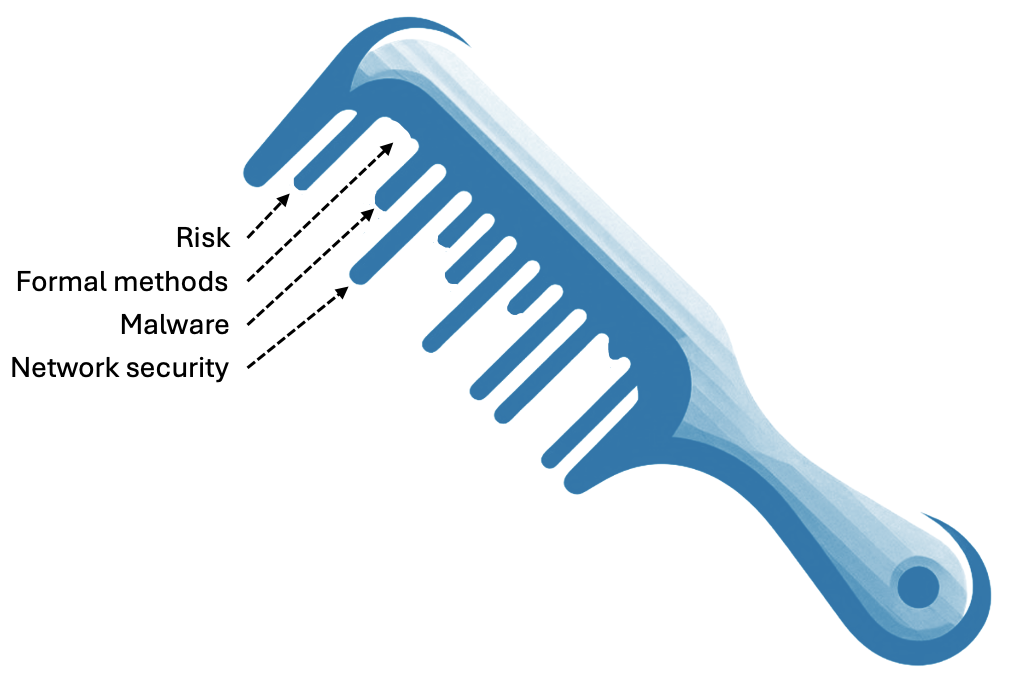
\includegraphics[keepaspectratio]{media/expertise_comb.png}}

}

\caption{The broken comb metaphor, which was suggested to us by John R.}

\end{figure}%

The survey used an interface based on a series of sliders through which
participants could express how they saw their own `broken combs' of
expertise, and to define similar `broken combs' reflecting the
combinations of expertise required to address cyber security problems
and challenges that they tackle in their work.

We based the `teeth' of the comb on the knowledge area classification
developed by the `CyBOK' project (Martin et al. 2021), extended slightly
to account for areas that are not accounted for in the standard CyBOK
classification (see
Section~\ref{sec-personal-expertise-within-and-beyond-cybok}).

We thus gathered three types of combs to support the analysis.

\begin{itemize}
\item
  The \textbf{personal comb} is just the values that a person put in for
  their own expertise using the sliders. For alignment calculations we
  only use the CyBOK values.
\item
  The \textbf{specialism comb} is a representation of the Cyber Careers
  Framework CyBOK mapping: we create these by assigning a numeric value
  to what the UKCSC considers to be `core', `related' or `wider'
  relevance to each specialism.
\item
  The \textbf{scenario comb} is the values that a person put in for that
  specific scenario using the sliders. For alignment calculations we
  only use the CyBOK values.
\end{itemize}

\subsection{The alignment metric
calculation}\label{the-alignment-metric-calculation}

In order to see how well (or badly) are two combs aligned, we compute an
\textbf{alignment index} \(A_{(x,y)}\) as follows.

Given a set of \textbf{test values} \(X:[x_0, x_1, ... x_n ]\) and a
corresponding set of \textbf{reference values}
\(Y:[y_0, y_1, ... y_n ]\), the alignment index will be:

\[
A_{(x,y)} = \frac{\sum I(X)}{\sum Y}
\]

Where the indicator function \(I(X)\) is defined as follows:

\begin{itemize}
\tightlist
\item
  \(I(X) = x_m\) when \(x_m \leq y_m\)
\item
  \(I(X) = y_m\) when \(x_m > y_m\)
\end{itemize}

The indicator function is used to prevent a test comb getting `credit'
for overshooting the reference values (which could otherwise
misleadingly offset deficits in other areas). To do so, it takes the
reference value as a ceiling in each tooth of the test comb. This also
means that the maximum possible alignment is 1.

With this, we will be calculating two types of alignments:

\begin{itemize}
\item
  \textbf{Personal alignment}, where test values (\(X\)) are the
  personal comb (responses) and the reference values (\(Y\)) are the
  specialism comb. This gives us a sense of how close respondents' combs
  are to the different kinds of specialism.
\item
  \textbf{Scenario alignment}, where test values (\(X\)) are the
  specialism comb and the reference values (\(Y\)) are the scenario
  comb. In this case, we are interested in how well the specialisms as
  defined in the Cyber Careers Framework provide the kind of expertise
  required to address each problem defined in the provided scenarios.
  For instance, if a problem scenario is defined by a respondent to
  require only expertise in Adversarial Behaviour and Forensics, the
  Cyber Security Management specialism would be best aligned of all the
  UKCSC specialisms, as this is the only specialism for which both of
  these knowledge areas are defined as `core' areas of expertise. We
  look at this for individual specialisms, and also look at the
  alignment of combinations of specialisms in permutations up to 5.
\end{itemize}

In both cases, the \textbf{alignment index} will result in a number
between \texttt{0} and \texttt{1}, where \texttt{1} means perfect
alignment between the test value and the reference value and \texttt{0}
means not aligned at all.

\marginnote{\begin{footnotesize}

Computations for the alignment metric can be audited at the file
\href{https://github.com/WarwickCIM/cyberexpertisediversity_survey/blob/main/scripts/alignment_metric.R}{\texttt{scripts/alignment\_metric.R}}

\end{footnotesize}}

\section{Results}\label{results}

The survey was conducted between 12/09/2024 and 19/11/2024 and received
responses from 56 individuals, describing 65 scenarios.

In this section we will be providing an overview of the responses
according to each of the blocks of the survey. Detailed analysis and
interpretations of those results can be found in the following sections
of the report and the appendices.

\subsection{Respondents' demographics}\label{respondents-demographics}

In terms of demographics, we can see (Table~\ref{tbl-responses-age})
that, more than 50\% of the responses are between 40 and 59 years old.

\begin{longtable}[]{@{}lrl@{}}

\caption{\label{tbl-responses-age}Responses by age}

\tabularnewline

\toprule\noalign{}
Age & N & Percent \\
\midrule\noalign{}
\endhead
\bottomrule\noalign{}
\endlastfoot
20-25 & 4 & 7.1\% \\
26-29 & 1 & 1.8\% \\
30-39 & 10 & 17.9\% \\
40-49 & 15 & 26.8\% \\
50-59 & 18 & 32.1\% \\
60 and over & 5 & 8.9\% \\
I prefer not to answer & 3 & 5.4\% \\

\end{longtable}

Table~\ref{tbl-responses-gender} and
Table~\ref{tbl-responses-transgender} shows a clear dominance of cis
male respondents over other genders. Cis female account for a 17.9\%,
and other genders are anecdotal in this survey.

\begin{longtable}[]{@{}lrl@{}}

\caption{\label{tbl-responses-gender}Responses by gender}

\tabularnewline

\toprule\noalign{}
Gender & N & Percent \\
\midrule\noalign{}
\endhead
\bottomrule\noalign{}
\endlastfoot
Male & 41 & 73.2\% \\
Female & 10 & 17.9\% \\
I prefer not to answer & 4 & 7.1\% \\
Non binary & 1 & 1.8\% \\

\end{longtable}

\begin{longtable}[]{@{}lrl@{}}

\caption{\label{tbl-responses-transgender}Responses by gender (2)}

\tabularnewline

\toprule\noalign{}
Trans & N & Percent \\
\midrule\noalign{}
\endhead
\bottomrule\noalign{}
\endlastfoot
No & 51 & 91.1\% \\
I prefer not to answer & 4 & 7.1\% \\
Yes & 1 & 1.8\% \\

\end{longtable}

In terms of ethnicity (Table~\ref{tbl-responses-ethnicity}), we can see
a clear dominance of White respondents (76.8\%), followed by far by
Asian and mixed race.

\begin{longtable}[]{@{}
  >{\raggedright\arraybackslash}p{(\linewidth - 4\tabcolsep) * \real{0.8736}}
  >{\raggedleft\arraybackslash}p{(\linewidth - 4\tabcolsep) * \real{0.0345}}
  >{\raggedright\arraybackslash}p{(\linewidth - 4\tabcolsep) * \real{0.0920}}@{}}

\caption{\label{tbl-responses-ethnicity}Responses by ethnicity}

\tabularnewline

\toprule\noalign{}
\begin{minipage}[b]{\linewidth}\raggedright
Ethnicity
\end{minipage} & \begin{minipage}[b]{\linewidth}\raggedleft
N
\end{minipage} & \begin{minipage}[b]{\linewidth}\raggedright
Percent
\end{minipage} \\
\midrule\noalign{}
\endhead
\bottomrule\noalign{}
\endlastfoot
White & 43 & 76.8\% \\
Asian (Indian, Pakistani, Bangladeshi, Chinese, any other Asian
background) & 4 & 7.1\% \\
Mixed two or more ethnic groups & 3 & 5.4\% \\
Prefer not to say & 3 & 5.4\% \\
Black/African/Caribbean & 1 & 1.8\% \\
Other (Arab or any others) & 1 & 1.8\% \\
NA & 1 & 1.8\% \\

\end{longtable}

In terms of disabilities (Table~\ref{tbl-responses-disabilities}),
respondents reporting some type of disability account for a total of
17.8\%.

\begin{longtable}[]{@{}
  >{\raggedright\arraybackslash}p{(\linewidth - 4\tabcolsep) * \real{0.8922}}
  >{\raggedleft\arraybackslash}p{(\linewidth - 4\tabcolsep) * \real{0.0294}}
  >{\raggedright\arraybackslash}p{(\linewidth - 4\tabcolsep) * \real{0.0784}}@{}}

\caption{\label{tbl-responses-disabilities}Responses by disabilities}

\tabularnewline

\toprule\noalign{}
\begin{minipage}[b]{\linewidth}\raggedright
Disabilites
\end{minipage} & \begin{minipage}[b]{\linewidth}\raggedleft
N
\end{minipage} & \begin{minipage}[b]{\linewidth}\raggedright
Percent
\end{minipage} \\
\midrule\noalign{}
\endhead
\bottomrule\noalign{}
\endlastfoot
No, I do not have a disability, or a history/record of having one & 45 &
80.4\% \\
I prefer not to answer & 6 & 10.7\% \\
Yes, I have a mental disability or neurodiversity, or have a
history/record of having one & 4 & 7.1\% \\
Yes, I have both a mental and physical disability, or have a
history/record of having them & 1 & 1.8\% \\

\end{longtable}

While the small sample, and opportunistic sampling approach prohibits
broader conclusions, these figures are broadly aligned with the sector
(National Cyber Security Centre 2021). We will argue, however, that the
data is suggestive that further data collection would be of value.

\subsubsection{Job-related questions}\label{job-related-questions}

In terms of job-related questions, we can see (
Table~\ref{tbl-responses-experience}) that half of our respondents have
less than 10 years of experience, despite most of responses being from
relatively mature respondees (see Table~\ref{tbl-responses-age}), and
71\% have up to 20 years. 12.5\% had more than 25 years of experience.
This is in line with the relatively high age of the respondents, but may
also suggest that some respondents may have shifted their career towards
cyber security less than 10 years ago.

\begin{longtable}[]{@{}lrl@{}}

\caption{\label{tbl-responses-experience}Responses by years of
experience}

\tabularnewline

\toprule\noalign{}
Age & N & Percent \\
\midrule\noalign{}
\endhead
\bottomrule\noalign{}
\endlastfoot
0-5 & 14 & 25.0\% \\
6-10 & 14 & 25.0\% \\
11-15 & 12 & 21.4\% \\
16-20 & 5 & 8.9\% \\
21-25 & 4 & 7.1\% \\
25+ & 7 & 12.5\% \\

\end{longtable}

\begin{longtable}[]{@{}lrl@{}}

\caption{\label{tbl-responses-org-size}Responses by organisation size}

\tabularnewline

\toprule\noalign{}
Organisation Size & N & Percent \\
\midrule\noalign{}
\endhead
\bottomrule\noalign{}
\endlastfoot
Large (250 employees or more) & 40 & 71.4\% \\
Medium (50 to 249 employees) & 5 & 8.9\% \\
Small (10 to 49 employees) & 5 & 8.9\% \\
Micro (1 to 9 employees) & 6 & 10.7\% \\

\end{longtable}

\begin{longtable}[]{@{}lrl@{}}

\caption{\label{tbl-responses-industry}Responses by Industry sector}

\tabularnewline

\toprule\noalign{}
Industry Sector & N & Percent \\
\midrule\noalign{}
\endhead
\bottomrule\noalign{}
\endlastfoot
Professional, Scientific, and Technical & 14 & 25\% \\
Information and Communications & 9 & 16.1\% \\
Utilities and Production (Including Manufacturing) & 9 & 16.1\% \\
Other (low n) & 8 & 14.3\% \\
Other (Please State) & 7 & 12.5\% \\
Education & 5 & 8.9\% \\
Transport and Storage & 4 & 7.1\% \\

\end{longtable}

\subsection{Comb responses}\label{comb-responses}

\begin{figure}

\centering{

\pandocbounded{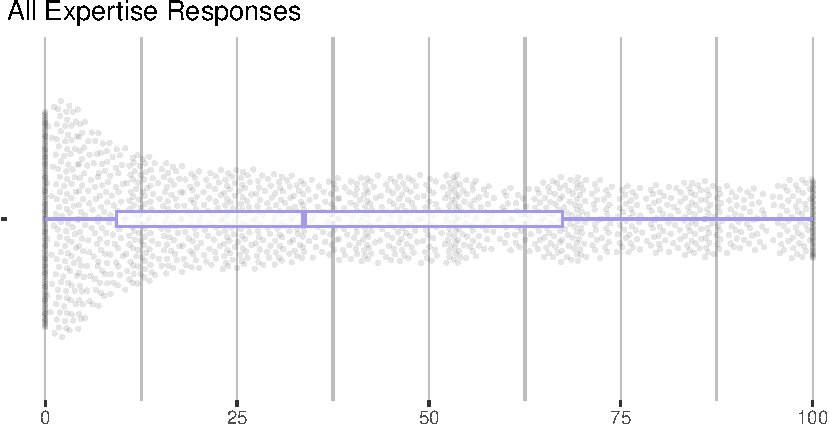
\includegraphics[keepaspectratio]{content/survey_files/figure-pdf/fig-personal-comb-aggregate-1.pdf}}

}

\caption{\label{fig-personal-comb-aggregate}Participants' responses on
their personal expertise combs, in aggregate}

\end{figure}%

\begin{figure}

\centering{

\pandocbounded{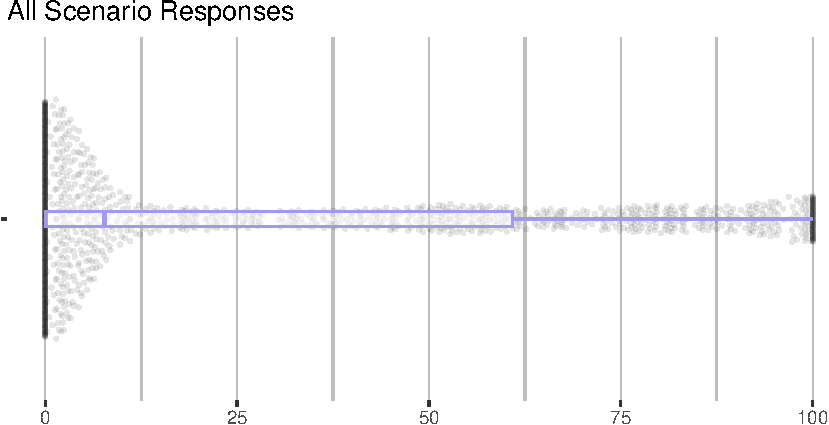
\includegraphics[keepaspectratio]{content/survey_files/figure-pdf/fig-scenario-comb-aggregate-1.pdf}}

}

\caption{\label{fig-scenario-comb-aggregate}Participants' responses on
their personal scenario combs, in aggregate}

\end{figure}%

The visualisations above are beeswarm plots overlaid with a box and
whisker plots showing all the responses in aggregate. For a more
detailed view, refer to \href{personal_combs.qmd}{Appendix A} and
\href{scenario_combs.qmd}{Appendix B}.

Figure~\ref{fig-personal-comb-aggregate} shows all the personal comb
responses. Respondents were using the full range of the sliders, with
10.1\% responses being set to 0 and 3.4\% set to 1.
Figure~\ref{fig-scenario-comb-aggregate} shows that respondents used the
full range of the sliders to specify the needs of scenarios, but tended
to leave more sliders at a low value when compared with personal combs.

Figure~\ref{fig-personal-comb-overall} below shows how the personal
score for each of the 26 categories was distributed. Breaking down the
responses by expertise category, we observe that our additional 5
non-CyBOK categories featured in respondents' profiles as commonly as
CyBOK categories did. This helps to validate that they were relevant and
recognisable.

\begin{figure}

\centering{

\pandocbounded{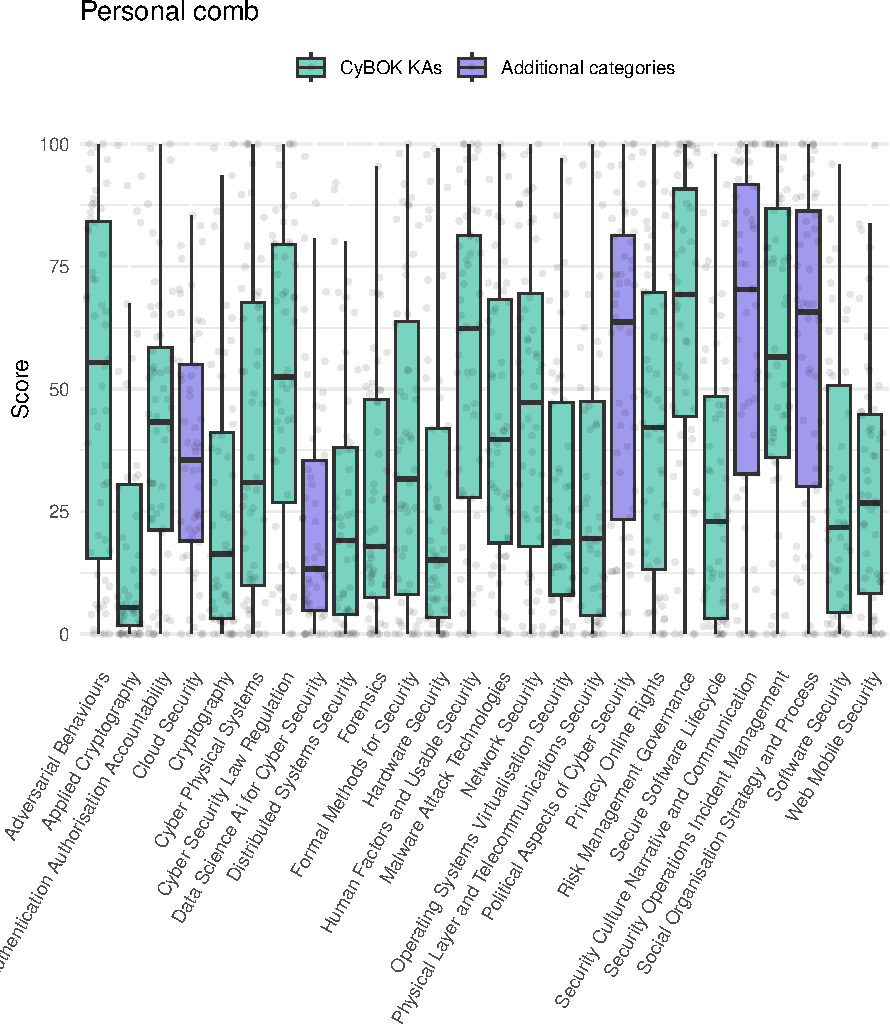
\includegraphics[keepaspectratio]{content/survey_files/figure-pdf/fig-personal-comb-overall-1.pdf}}

}

\caption{\label{fig-personal-comb-overall}Overall distribution of
personal comb scores (blue: CyBOK KAs; green: additional categories)}

\end{figure}%

Figure~\ref{fig-scenario-comb-overall} shows that when describing
scenarios, respondents tended to use a subset of the `teeth' and the
other sliders at a low value. The scenarios elicited from respondents
favoured areas such as \emph{security culture}, \emph{adversarial
behaviours}, \emph{risk management} and \emph{security operations}. This
reflects the prominence of organisational challenges and incidents in
the dataset.

\begin{figure}

\centering{

\pandocbounded{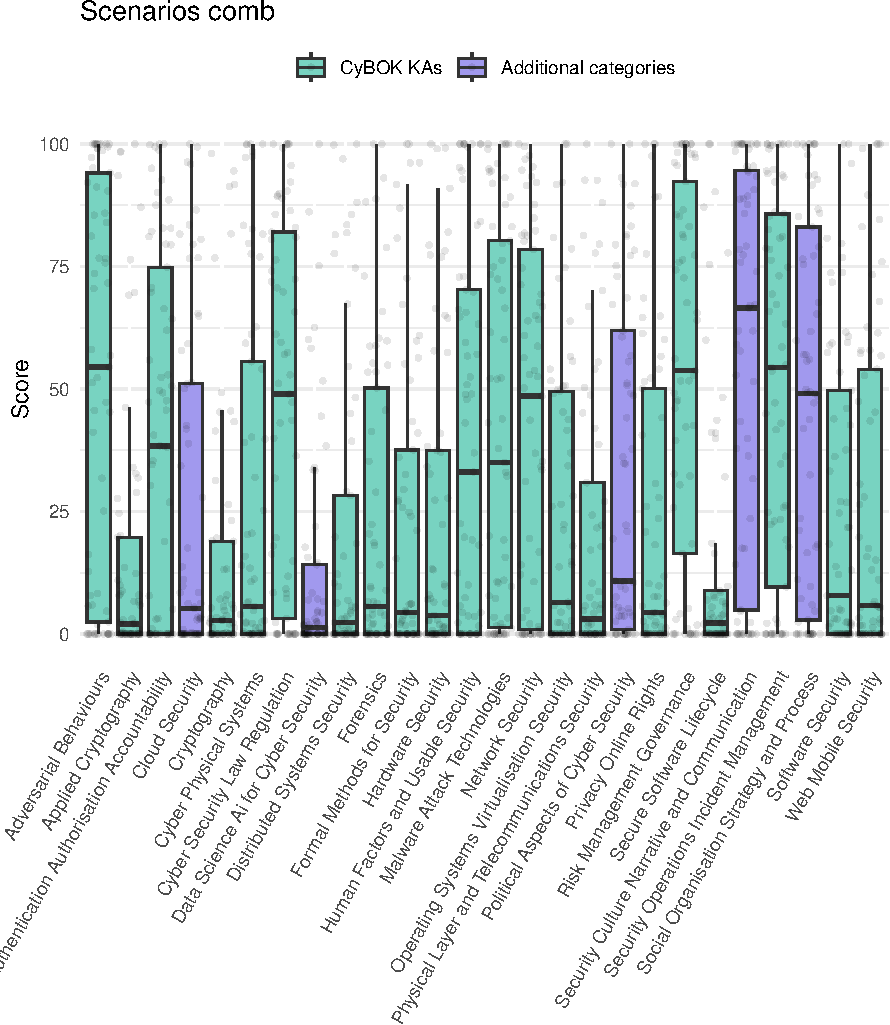
\includegraphics[keepaspectratio]{content/survey_files/figure-pdf/fig-scenario-comb-overall-1.pdf}}

}

\caption{\label{fig-scenario-comb-overall}Overall distribution of
scenarios comb scores by category}

\end{figure}%

\section{Key limitations}\label{key-limitations}

Given resource constraints (we received no direct funding for this
research), the project was conceived as an exploratory exercise, aiming
to develop analytical tools suitable for investigating the value of
diverse expertise in cyber security in the UK. It is important to bear
in mind the following key limitations when interpreting the results.

\subsection{Sampling}\label{sec-sampling}

The total number of responses is modest (56). To put this into context,
the Decrypting Diversity 2020 report was based on 1252 responses, and
the 2021 follow-up drew on a sample of 945.

Our sampling strategy was opportunistic: we distributed the invitation
to participate via a number of cyber security related industry networks
within the UK and on LinkedIn. A larger, random-sampling approach would
have many benefits but would require much more significant investment. A
convenience approach was chosen as appropriate for exploratory analysis
demonstrating the value of an analytical frame that brings questions
about the distribution and value of diverse expertise into conversation
with questions about diversity of personal characteristics. Small sample
studies like this should be seen as part of the wider endeavour to
understand the domain, as opportunities for lightweight prototyping of
methodologies for data collection and analysis.

\subsection{Sliders}\label{sliders}

Given the challenges in establishing an absolute scale across all
`teeth', we asked participants to focus on the relative proportions of
each category, the focus thus being on the `shape' of expertise rather
than its absolute extent. Because sliders generate numerical values,
they allow for analysis of these shapes, at individual or aggregate
levels, but it must be remembered that the scales being applied are
inevitably imprecise.

Because CyBOK is designed to refer to established areas of cyber
security knowledge, we assumed participants would be familiar with the
categories, and able to provide a relative assessment of their own
expertise. However, respondents will vary in their level of
understanding of the CyBOK categories, and this will also introduce
imprecision into the analysis. A better resourced survey might assess
familiarity with the categories as part of the survey process, or single
out a subset of respondents for an interview to examine levels of
understanding.

\subsection{Alignment scores}\label{alignment-scores}

The data has some important limitations that should be kept in mind when
interpreting alignment scores:

\begin{itemize}
\item
  The specialisms are defined according to `core', `related' and `wider'
  relevance of categories of expertise, which to be used in our
  calculations have to be translated into positions in the slider. We
  have chosen values of 90, 60 and 30 as parameters for these levels of
  relevance respectively. Alternative parameters can be readily
  substituted in the calculation.
\item
  The specialisms are defined according to the standard CyBOK knowledge
  area classification. The relevance of other forms of expertise is left
  undefined. This means that our additional teeth of the comb,
  representing areas that are not accounted for in CyBOK, must be
  ignored for the purposes of the alignment calculations. In certain
  cases, for instance where a scenario required significant amounts of
  expertise in one or more of the non-CyBOK areas, the alignment
  calculation could be misleading. We have highlighted this in the
  analysis, and reflect on how reliance on established classifications
  like CyBOK creates challenges where one is interested in accounting
  for neglected or emerging areas of expertise.
\end{itemize}

\bookmarksetup{startatroot}

\chapter{Professionalisation and
Inclusion}\label{professionalisation-and-inclusion}

\section{Professionalizing Cyber Security in the
UK}\label{professionalizing-cyber-security-in-the-uk}

Concerns about the adequacy of the UK's cyber security workforce, and
its ability to protect society, state and economy, have driven a number
of interconnected policy efforts, aiming to:

\begin{itemize}
\item
  formalize cyber security education,
\item
  bring more people into the field,
\item
  give recognition to those with cyber security expertise,
\item
  to ensure that adequate cyber security knowledge is integrated into
  related professions, and
\item
  to enable employers to better understand what they need from their
  cyber security employees.
\end{itemize}

The first UK National Cyber Security Strategy, published in 2016,
identified the need for government to do more to support the development
of the cyber security profession\footnote{\url{https://www.gov.uk/government/publications/national-cyber-security-strategy-2016-to-2021}}.
As part of the implementation of the Strategy, in 2018, the Department
for Digital, Culture, Media and Sport launched a proposal and
consultation on the creation of the UK Cyber Security Council (UKCSC).
The consultation recognised that there were existing forms of
recognition, such as offered by the Institute of Information Security
Professionals, which received a Royal Charter in 2018, and the
International Information System Security Certification Consortium
(ISC2), which governs the international CISSP (Certified Information
Systems Security Professional) qualification, but argued that there were
outstanding issues with coverage (some kinds of cyber security expertise
were not covered, or partially covered), and equivalence. The UKCSC was
thus set up to ``act as a governing voice for the cyber security
profession in the UK'' (Ministry of Defence 2021), and was launched in
2021.

Pillar 5 of the UK National Cyber Security Strategy 2022-2030, is the
objective to `develop the right cyber security skills, knowledge and
culture' so that `sufficient, skilled and knowledgeable professionals
fulfil all required cyber security needs' (Cabinet Office 2022). This is
to be delivered through ``consistent taxonomies, standards and
pathways'' providing ``diverse and fulfilling cyber security careers''
and wider status recognition through accreditation and standardisation.
The UKCSC's work has thus become central to the national strategic
vision.

In pursuit of these goals, the UKCSC developed a `Cyber Careers
Framework' which identifies four levels of expertise (Associate,
Practitioner, Principal, and Chartered) across a set of 15 specialisms.
Assessments of applicants for recognition are carried out by member
organisations of UKCSC, who receive a license for specific specialisms:
currently the Chartered Institute of Information Security, The Cyber
Scheme, and CREST. Recognition is being delivered in a phased manner,
and the first chartered cyber security professionals (ChCSP) were
recognised in October 2023. The roll-out process has met with some
difficulties, with only 6 specialisms currently available, and a
relatively low uptake so far. One challenge has been in the definition
of specialisms, as some of these were inherited from pre-existing
schemes such as the NCSC's Certified Cyber Professional\footnote{\url{https://www.ncsc.gov.uk/news/forthcoming-closure-of-ccp-scheme}},
whereas others have been defined from scratch. This has led to some
inconsistencies in the style and extent of requirements across
specialisms. It is widely recognised that the Cyber Careers Framework
will need to evolve and improve over time, something that is necessary
in any case to keep pace with changing technologies, threats and
practices. Gathering and interpreting data will be important in enabling
a responsive approach to cyber security problems and practices, on its
workforce and the distribution of expertise, in order to maintain its
alignment and relevance in the years ahead.

\section{Social closure}\label{social-closure}

Professionalisation can be analysed sociologically through the lens of
social openness and social closure. The concept of social relationships
being `open' or `closed' has deep roots in sociology, and is a building
block of Max Weber's classic analysis of social action (Weber 2019).
Social closure is an umbrella term for the ways in which groups
construct and maintain monopolies over opportunities, by including some
people and excluding others. Understanding how and why closure occurs is
key to our understanding of social structure and power. It can operate
at multiple levels. Even where opportunities are formally open, groups
may nevertheless be able to maintain control over resources through
influencing access to jobs or status, for instance through cronyism or
nepotism. Closure can create durable barriers to entry or `glass
ceilings' that limit opportunities. Social closure can be durable
because, once they exist, monopolies on resources tend to create an
alignment of interest among group members, as they have a common
interest in maintaining the status quo and resisting change. Weber
considered guilds to be an `archetype' of closure where it is motivated
by a cooperative monopolisation of (resource) acquisition, and under the
rubric of `occupational closure' the sociology of professions has
studied professionalisation as an important example of social closure in
the modern age.

There is a tension between occupational closure and the values of social
liberalism that promote fair access and equality of opportunity. In the
cases of the professions, the justification of occupational closure
involves achieving a balance between competing moral principles: on the
one hand, for buildings to be safe, for accounts to be trustworthy, for
all to have fair and equal representation under the law, for healthcare
to be safe, and so on, it is necessary to restrict who can practice
engineering, accountancy, law and medicine to those who have met a
certain standard of qualification and committed to accepted standards of
conduct. On the other hand, while entry into these professions may be
formally open and non-discriminatory, entrants often need considerable
capital---social capital in the form of social networks giving access to
opportunities for apprenticeships and experience, cultural capital in
the form of the ability to `fit in,' be `taken seriously' and generally
navigate within professional communities, and financial capital in the
form of resources to support what are often extended periods of training
or low pay at the start of careers---and so the institutional structure
of the professions tends to reinforce existing social inequalities. It
is not by accident that the traditional British middle classes are
commonly referred to as `the professional class'. Professional bodies,
such as the British Medical Associations, the Law Society, the
Association of Chartered Certified Accountants, and so on, thus tend to
understand their mission as having two sides: one that focuses on
ensuring standards of competence and conduct are met, and the other
intervening to improve and support equitable access to the profession,
through special initiatives, financial support, community engagement,
communication campaigns, and research. In short, professional bodies'
interest in equality, diversity and inclusion should not be seen as a
separate side project, but as a core project that ensures the social
legitimacy of occupational closure, by ensuring and demonstrating that
the profession is a vehicle for, and not an obstacle to, fair access.

The success of the project to professionalise cyber security in the UK
will depend on the ongoing legitimacy of bodies such as the UKCSC. Cyber
security is a young profession, and legitimacy cannot rest on a received
understanding of its members as an elite group (as is arguably the case
with doctors or lawyers). It is crucial to show how diversity will be
understood and managed in the years ahead, so that achievement can be
celebrated, and so that the contribution of diversity to the delivery of
cyber security outcomes is part of the vision for the sector. This will
require that professional bodies are attentive to, and responsive to,
challenges of diversity.

\section{The value of diversity}\label{the-value-of-diversity}

While considerations of social closure are sufficient to illustrate why
diversity is a core priority for the legitimacy of the UKCSC, an even
stronger argument can be constructed based on research into the value of
diversity. Sociologists have argued that organisational or institutional
diversity has value as a resource during times of economic transition
(Grabher and Stark 1997). Scholars in safety studies have argued that
overly homogeneous patterns of reasoning and valuation can `incubate
disaster', a central problem for organisations that operate in safety
critical contexts (Dekker and Pruchnicki 2014; Vaughan 1996). In Karl
Weick's classic studies of high reliability organisations, diversity can
be understood as a source of `requisite variety' that enables
organisations to avoid accidents.

\begin{quote}
Whether team members differ in occupational specialities, past
experience, gender, conceptual skills, or personality may be less
crucial than the fact that they do differ and look for different things
when they size up a problem. If people look for different things, when
their observations are pooled they collectively see more than any one of
them alone would see. However, as team members become more alike, their
pooled observations cannot be distinguished from their individual
observations, which means collectively they know little more about a
problem than they know individually (Weick 1987).
\end{quote}

Several studies have indicated that hiring people from diverse
backgrounds provides value in broadening organisational repertoires of
thought and practice, and enhancing the potential to innovate (Herring
2009). Researchers have also argued that homogeneity can be a source of
problems, with evidence, for instance, that homogeneity leads to bubbles
and inefficient markets (Levine et al. 2014). The 2020-2021 NCSC/KPMG
Decrypting Diversity reports explicitly reference this line of thinking,
arguing that diversity in the workplace brings ``benefits including
better financial performance, increased creativity and innovation,
greater employee satisfaction, lower absenteeism and stronger talent
retention'' (NCSC 2020). In other words, diversity is valuable not just
because inequality and discrimination are unacceptable, but also because
it is a driver of innovation and ultimately a more secure society.

\section{The status quo}\label{the-status-quo}

The `Decrypting Diversity' reports painted a mixed picture of diversity
in the cyber security profession. On the one hand, the proportion of the
cyber profession that identifies as coming from a BAME (Black and
Minority Ethnic) background, and the proportion that identifies as
Lesbian, Gay and Bisexual (LGB), were broadly in line with national
figures. Data on Trans people was insufficient to make reliable claims,
and more research is needed in areas such as this. Gender is
well-recognised to be an issue for cyber security, with survey
respondents identifying as male outnumbering those identifying as female
2:1 in the Decrypting Diversity studies. Here, the cyber security
profession needs to engage with broader efforts, as the same gender
imbalance is found across the technology workforce. Socio-economic
backgrounds were also skewed, for instance with those who had attended
private schools over-represented. Furthermore, even in areas such as
ethnicity or sexuality, where the profession was broadly in line with
the general population, survey respondents noted that people from BAME
backgrounds or who identified as LGB were more likely to have faced
discrimination in the workplace.

The Decrypting Diversity report focuses on the experiences of people
within the cyber security profession, and although it was intended to be
part of a series of annual studies, only two were carried out. Some of
this research was folded into the `Cyber Security Skills in the UK
Labour Market Survey'\footnote{\url{https://www.gov.uk/government/publications/cyber-security-skills-in-the-uk-labour-market-2025/cyber-security-skills-in-the-uk-labour-market-2025\#diversity-in-cyber-security-1}},
and like Decrypting Diversity, these ongoing surveys focus on individual
diversity, and do not address connections with diversity of expertise,
either at the personal level or at the level of the key problems that
the cyber security profession is expected to address in work contexts.
They do, however, point to the need for further research. The 2025 Cyber
Security Skills in the UK Labour Market Survey pointed, for instance, to
concerning indications that ethnic diversity has been trending downwards
within senior cyber security roles, from 15\% in 2021, to 8\% in 2025.

Diversity of expertise is less well studied than individual diversity in
cyber security, though recent work building on the CyBOK framework is
aiming to address this. Developing a `knowledge profiling' approach,
Nautiyal and Rashid propose a tool for organisations to assess their
internal expertise, key certifications, and expertise brought by partner
organisations (Nautiyal and Rashid 2024). Other recent work uses CyBOK
to analyse the `cyber skills gap' through the analysis of job adverts
(Attwood and Williams 2023). The Cyber Expertise Diversity Survey was
developed in this vein. Like these studies, we focus on the
methodological possibilities, examining how the diversity of expertise
may be made visible and actionable. Our approach aims to make
connections between diverse profiles of expertise among professionals,
professional frameworks, and the alignment of both of these with problem
scenarios.

\section{Data analysis}\label{data-analysis}

\subsection{Alignment of respondents with the
specialisms}\label{alignment-of-respondents-with-the-specialisms}

The visualisation below shows an overall view of how our respondents
aligned with the UKCSC specialisms. The variance was relatively modest,
with the highest average alignment roughly double that of the lowest
average alignment. Looking at the individual boxplots, we note that our
sample spanned a wide range, including respondents that scored very
highly and very low in each area.

\begin{figure*}

\centering{

\pandocbounded{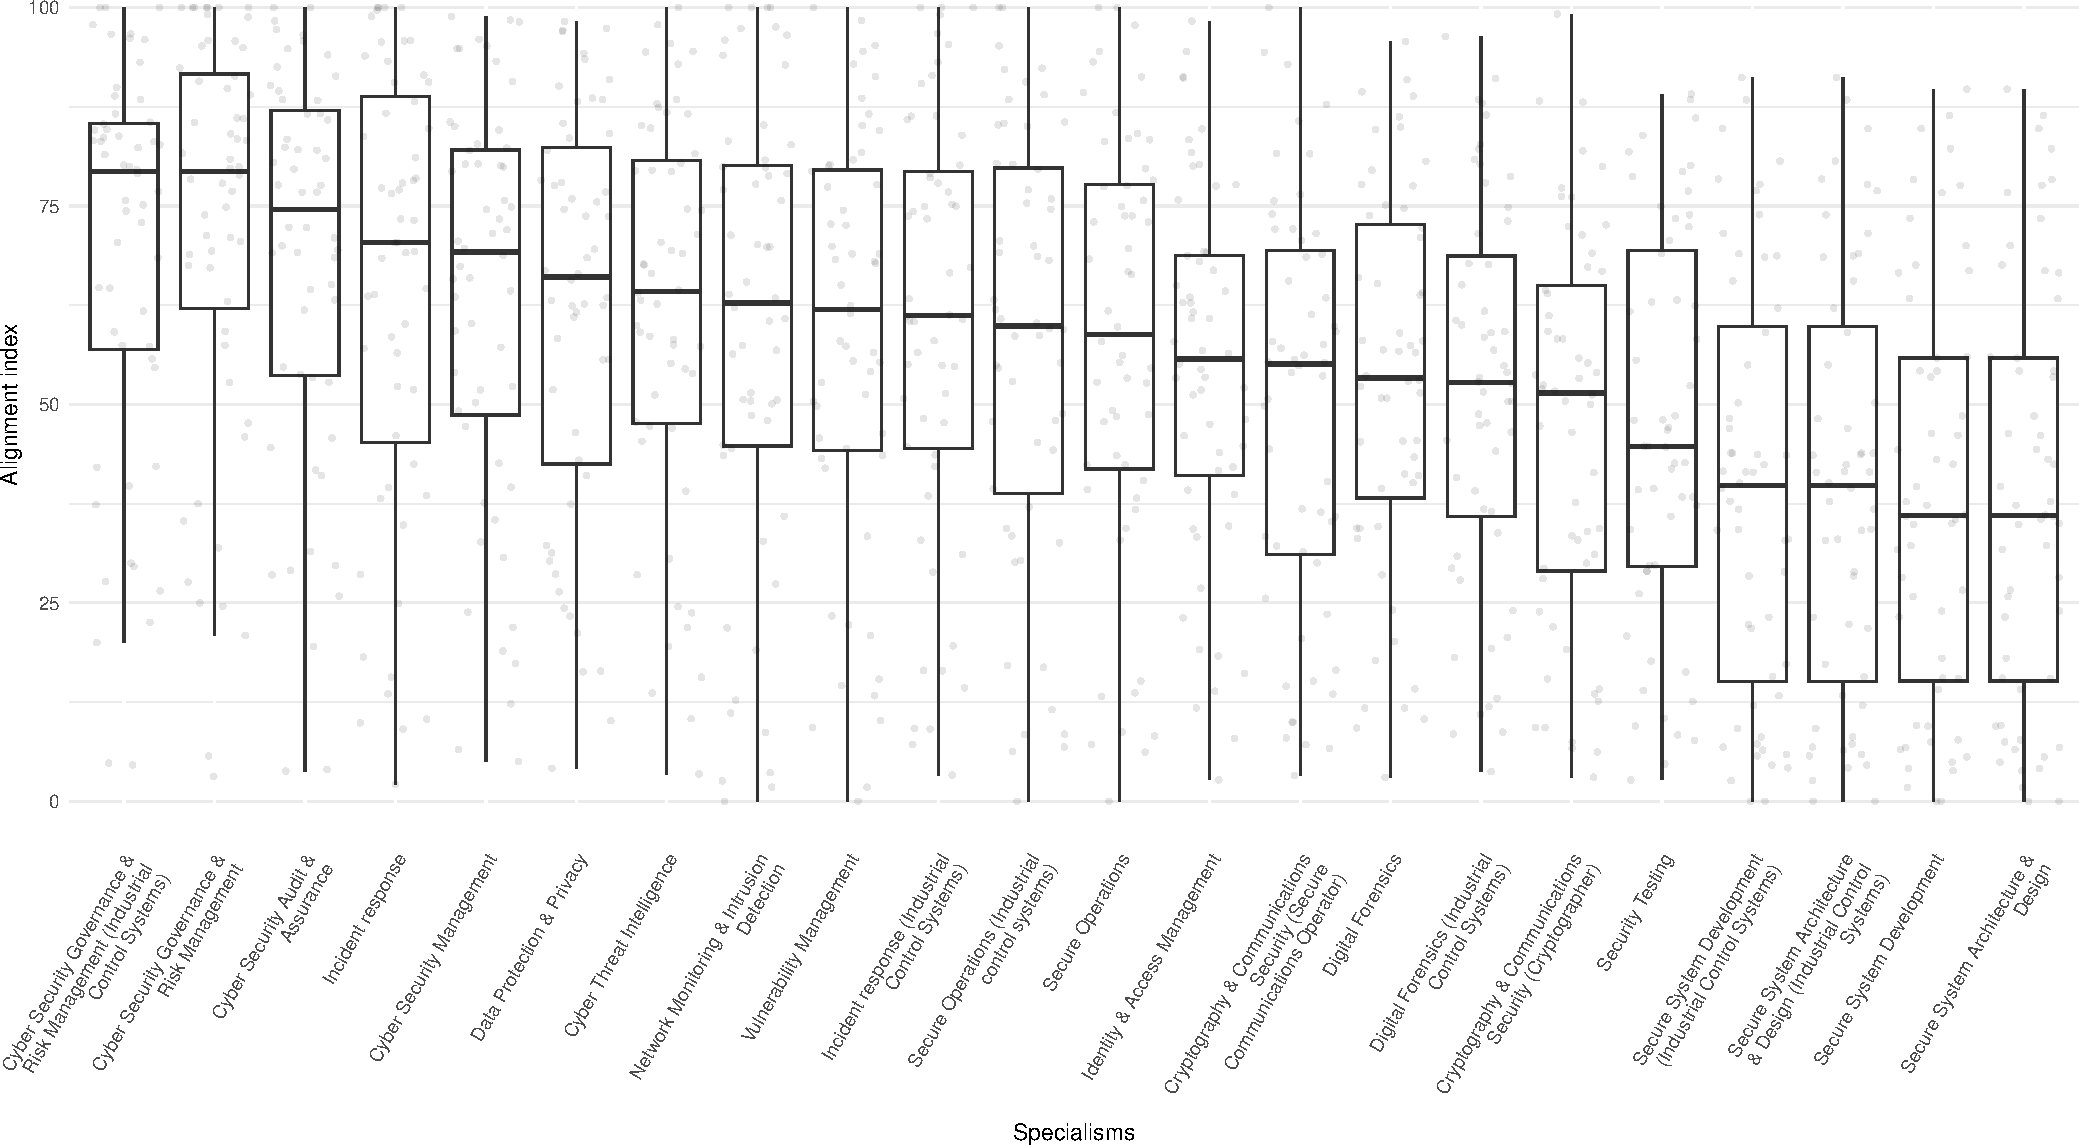
\includegraphics[keepaspectratio]{content/professionalisation_files/figure-pdf/fig-personal-alignment-scenario-1.pdf}}

}

\caption{\label{fig-personal-alignment-scenario}Personal alignment to
specialism}

\end{figure*}%

Of particular interest for our analysis is breaking down the overall
picture according to key attributes.

\subsection{Alignment based on key
attributes}\label{alignment-based-on-key-attributes}

\subsubsection{Gender}\label{gender}

When we break out alignment by gender we notice that people identifying
as men were on average better aligned than those identifying as women or
non-binary in all areas apart from \emph{Cyber security audit and
assurance}, \emph{Cyber security governance and risk management} and
\emph{Data protection and privacy}. We have ignored `prefer not to say'
in this case.

\begin{figure*}

\centering{

\pandocbounded{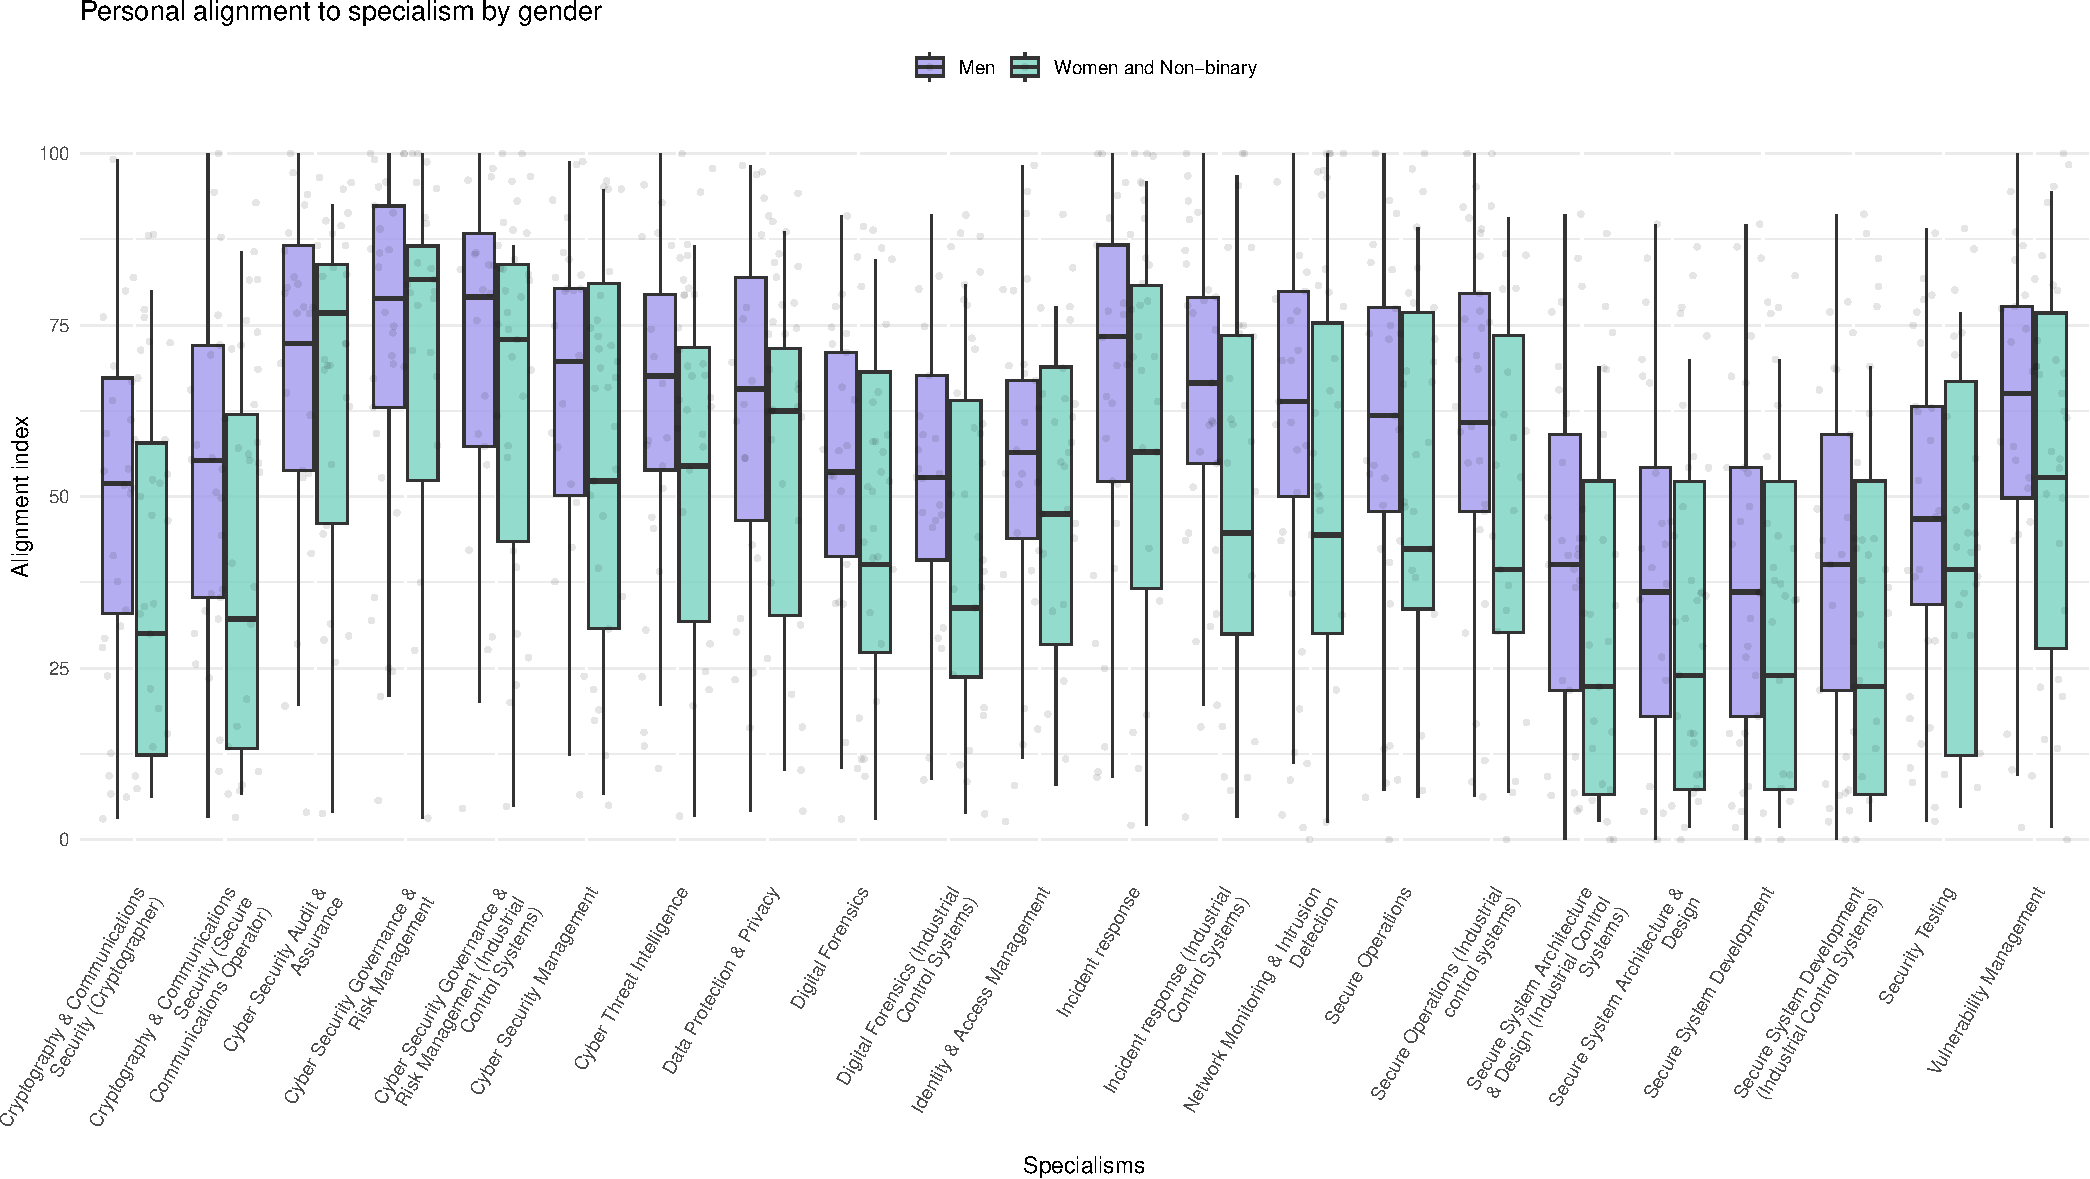
\includegraphics[keepaspectratio]{content/professionalisation_files/figure-pdf/fig-personal-alignment-scenario-gender_v2-1.pdf}}

}

\caption{\label{fig-personal-alignment-scenario-gender_v2}Personal
alignment to specialism by gender}

\end{figure*}%

\subsubsection{Age}\label{age}

The same view but broken down by age shows that, interestingly, in our
sample younger respondents were not less well aligned than older
respondents. This could reflect the fact that younger cyber security
professionals may have studied degrees relating to cyber security that
did not exist when older respondents were students (degrees that have
syllabuses that aim at comprehensive coverage). Understanding this view
from a larger dataset would be illuminating about how the profile of the
profession is changing.

\begin{figure*}

\centering{

\pandocbounded{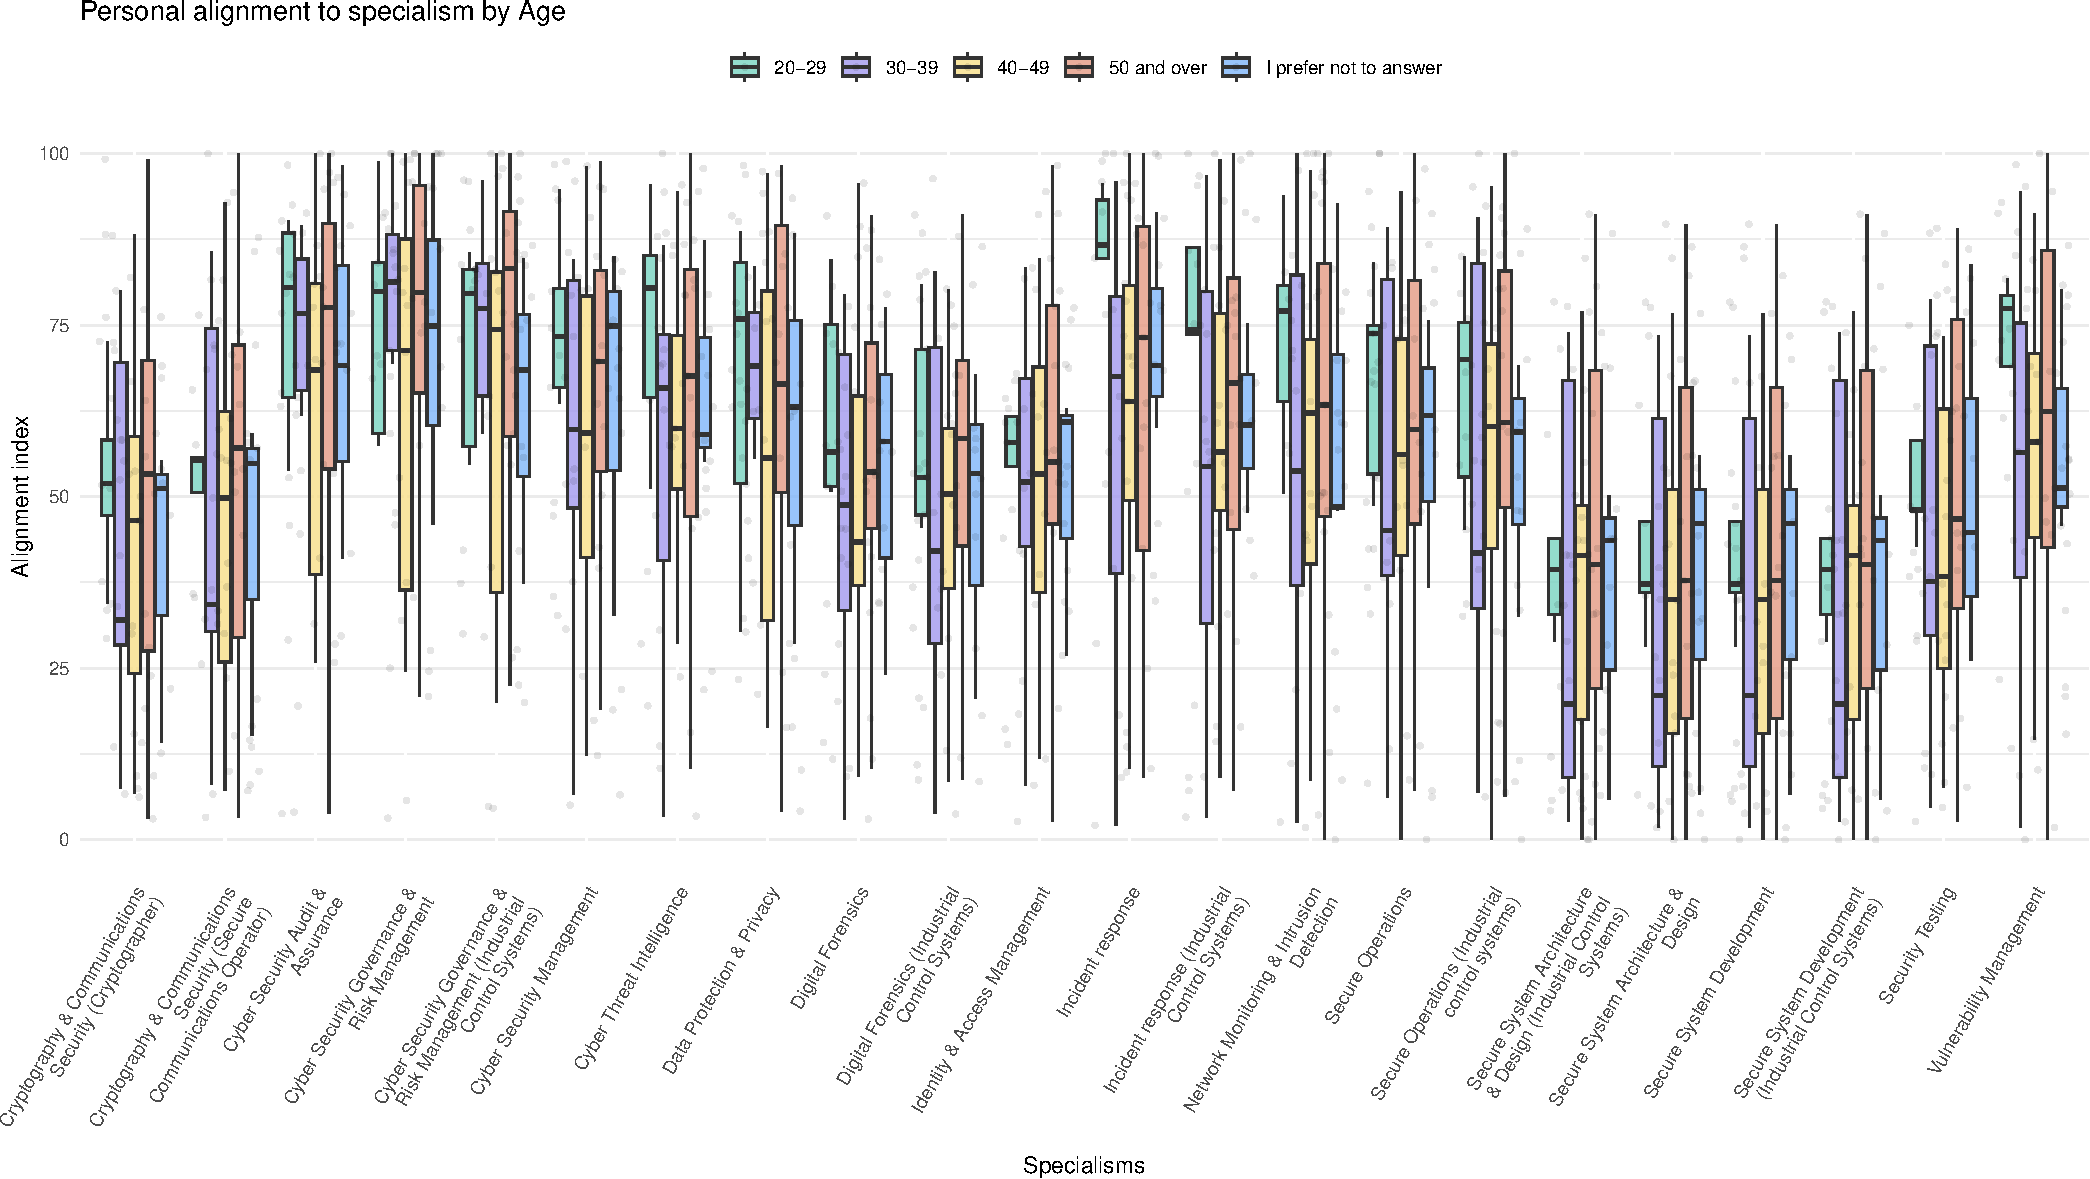
\includegraphics[keepaspectratio]{content/professionalisation_files/figure-pdf/fig-personal-alignment-scenario-age_v2-1.pdf}}

}

\caption{\label{fig-personal-alignment-scenario-age_v2}Personal
alignment to specialism by age}

\end{figure*}%

\subsubsection{Sexual orientation}\label{sexual-orientation}

In the visualisation below, respondents were asked `Do you identify as
lesbian, gay or bisexual?'.

\begin{figure*}

\centering{

\pandocbounded{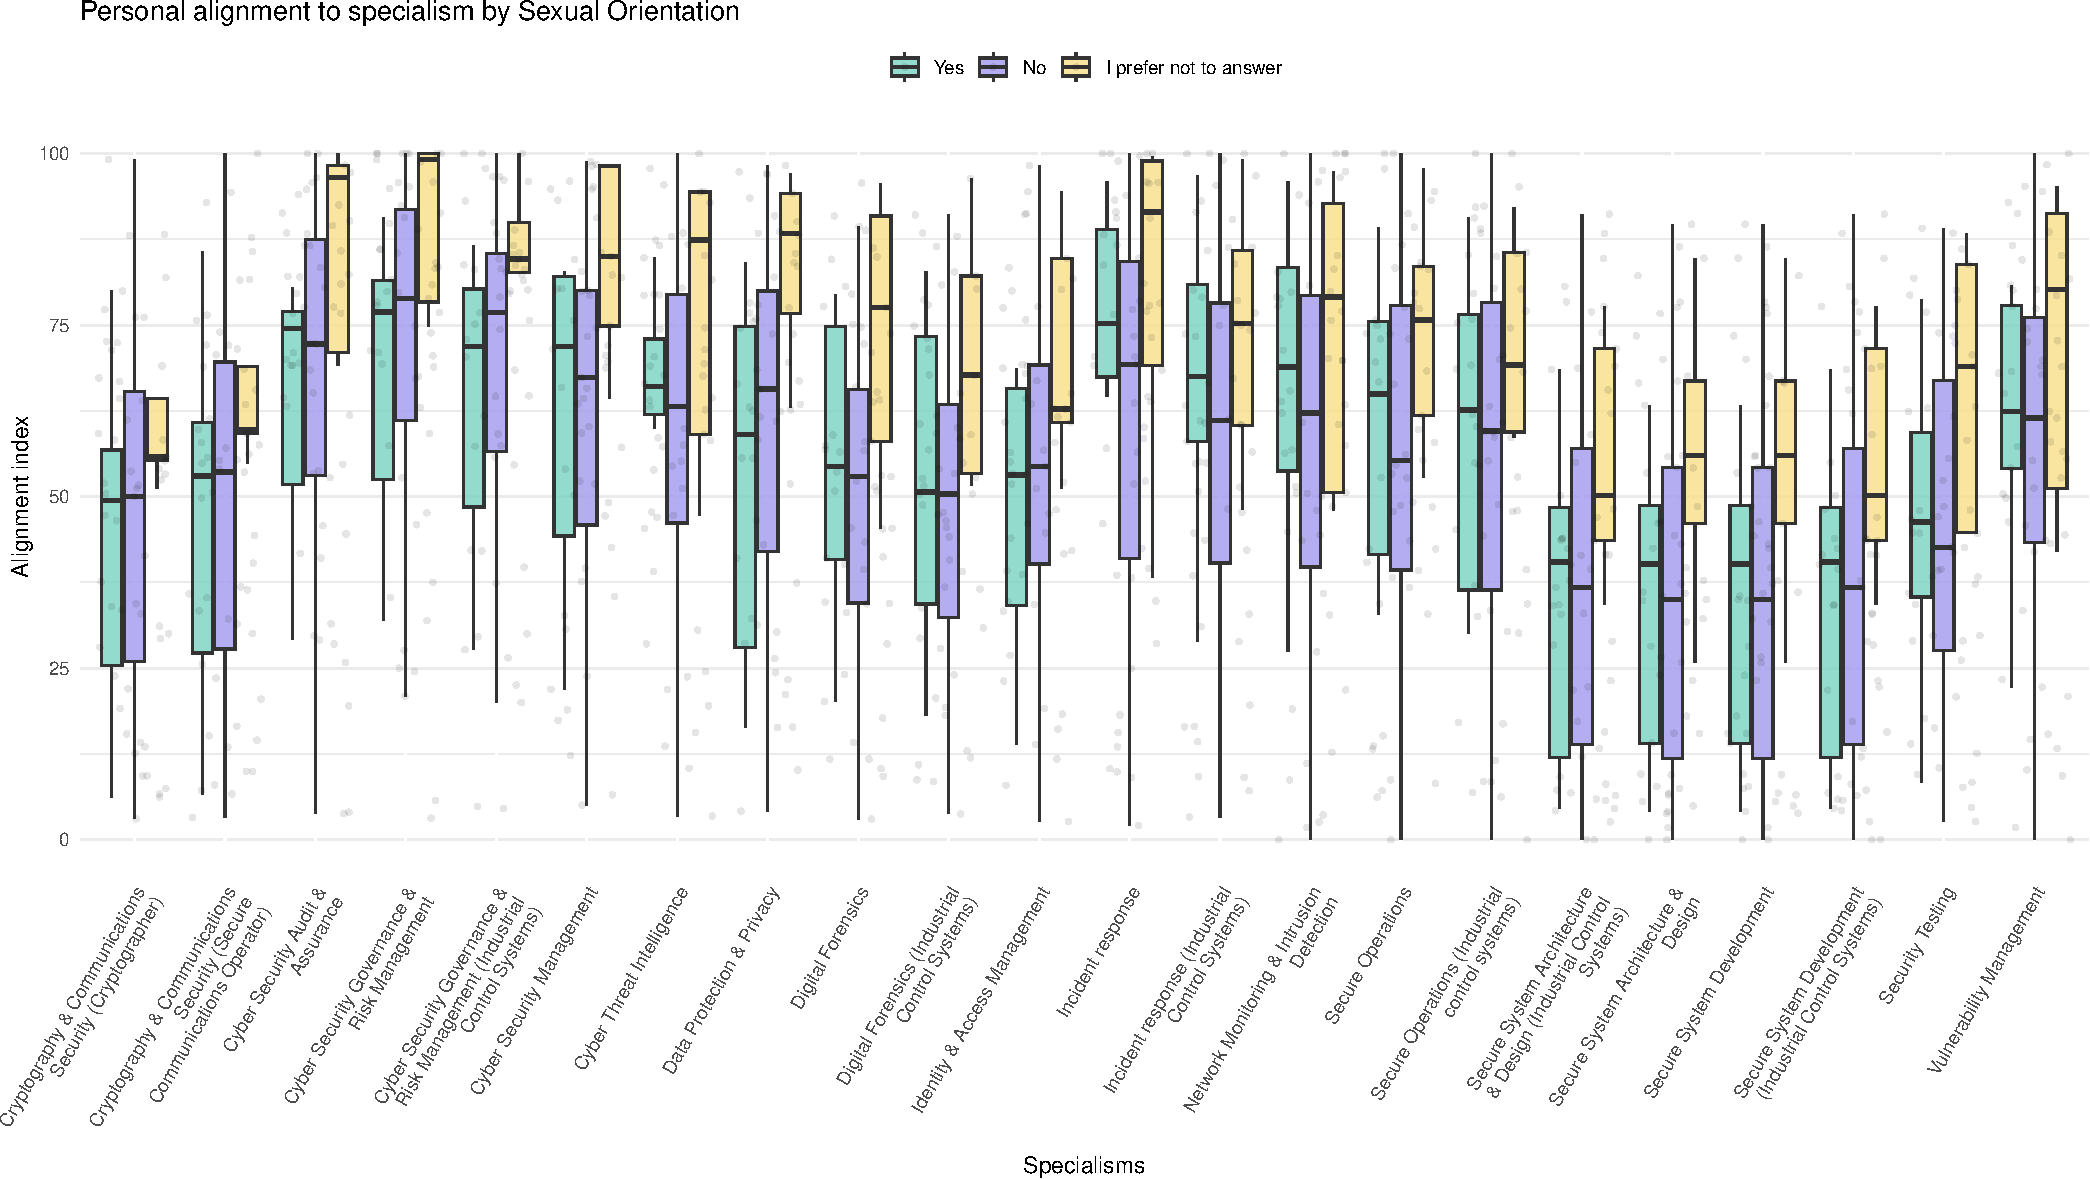
\includegraphics[keepaspectratio]{content/professionalisation_files/figure-pdf/fig-personal-alignment-scenario-sexual-orientation_v2-1.pdf}}

}

\caption{\label{fig-personal-alignment-scenario-sexual-orientation_v2}Personal
alignment to specialism by sexual orientation}

\end{figure*}%

Our study shows encouraging indicative results that sexual orientation
does not significantly map on to differences in alignment with
specialisms.

\subsubsection{Ethnicity}\label{ethnicity}

Due to having a low number of respondents in some categories, we've
grouped data into three main categories: white, Asian and `all other
ethnicities'.

\begin{figure*}

\centering{

\pandocbounded{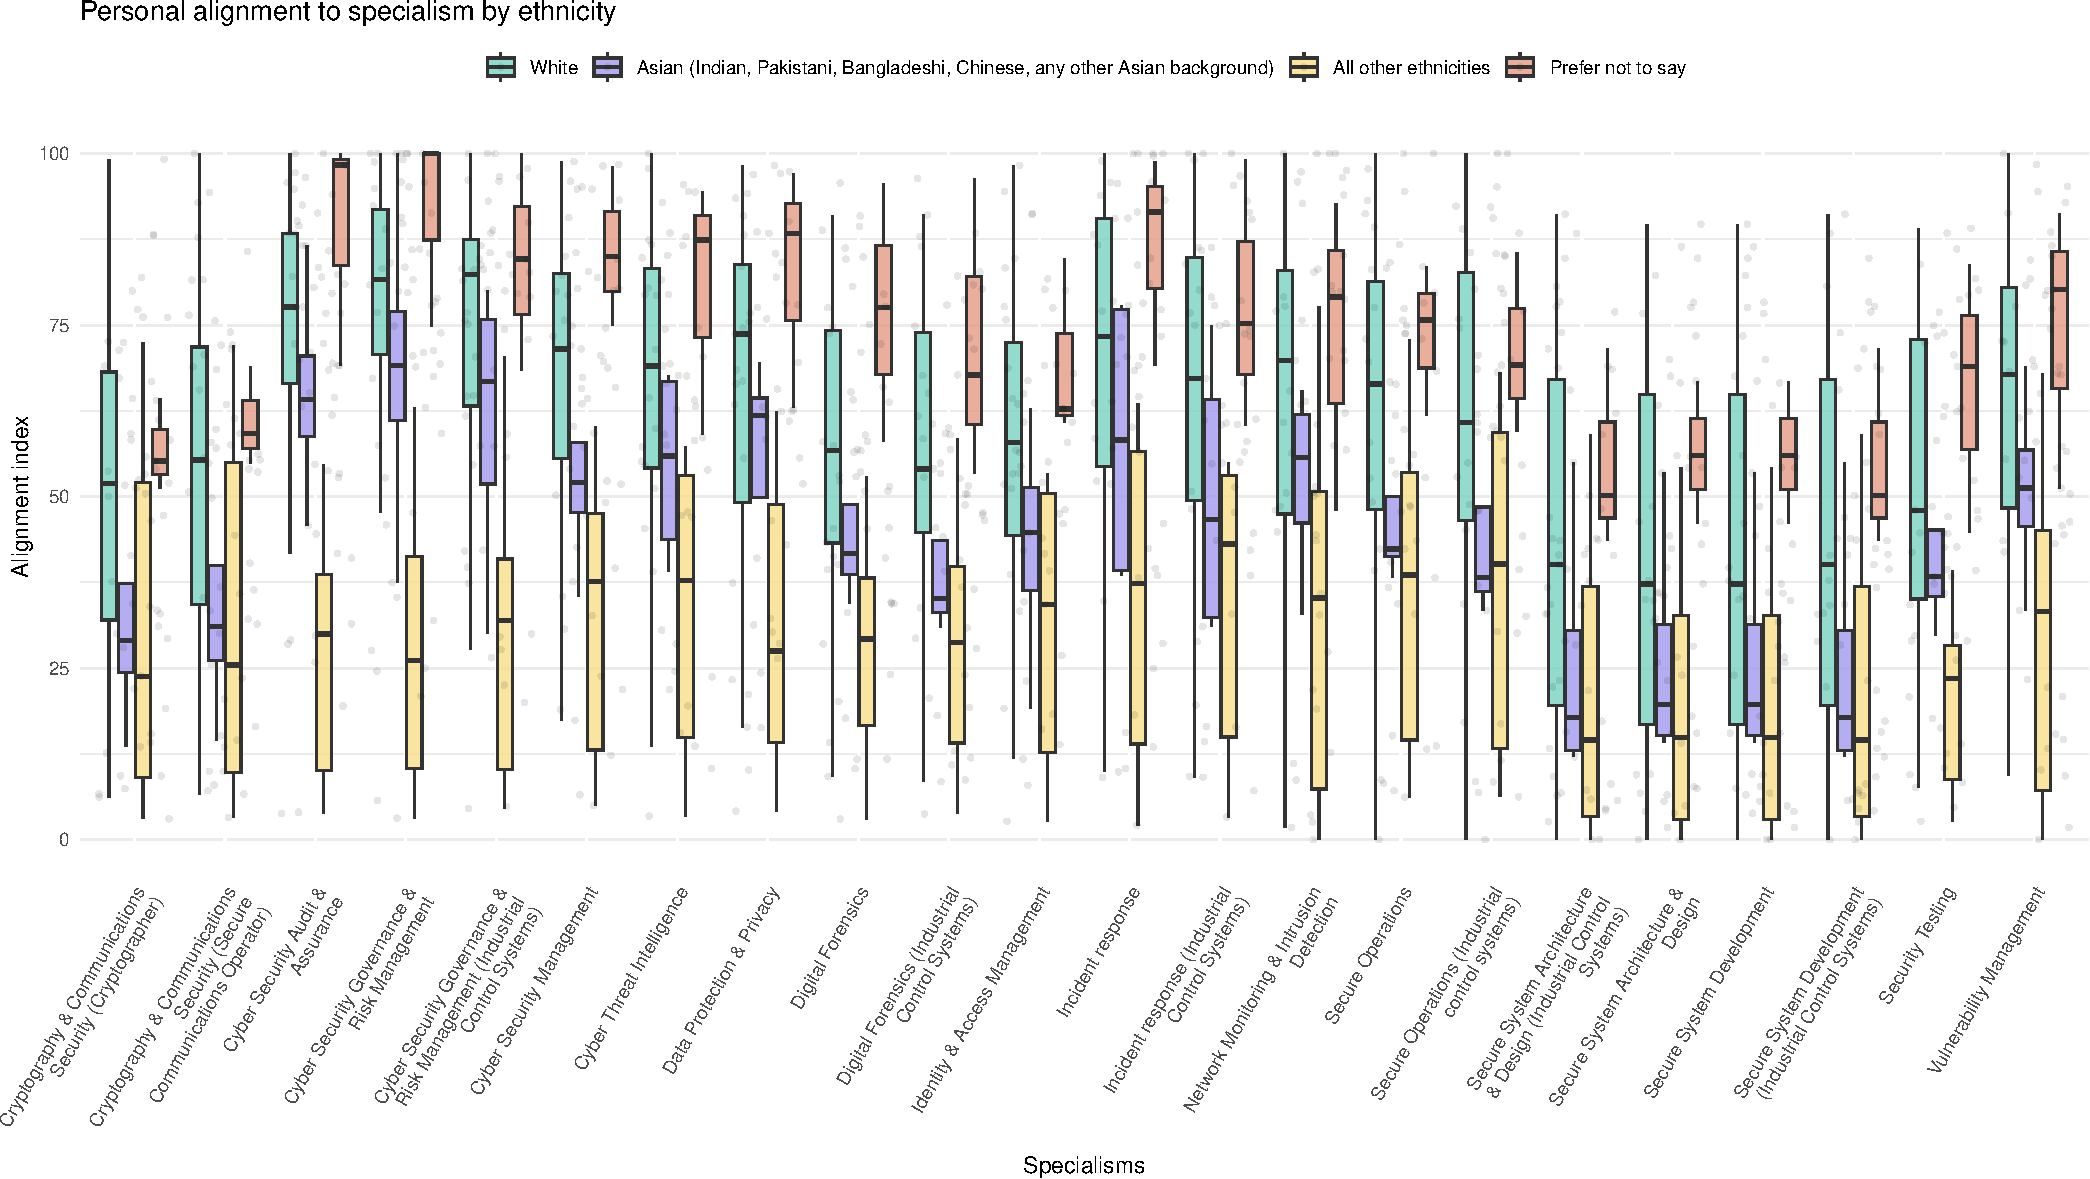
\includegraphics[keepaspectratio]{content/professionalisation_files/figure-pdf/fig-personal-alignment-scenario-ethnicity_v2-1.pdf}}

}

\caption{\label{fig-personal-alignment-scenario-ethnicity_v2}Personal
alignment to specialism by ethnicity}

\end{figure*}%

It is potentially concerning to observe that respondents identifying as
white were, on average, most well aligned with every single specialism.
This observation alone could justify further research.

\subsubsection{Further analysis}\label{further-analysis}

The suggestive patterns we observe, particularly in relation to gender
and ethnicity, warrant further investigation in order to investigate the
explanation. Candidate factors include:

\begin{enumerate}
\def\labelenumi{\arabic{enumi}.}
\item
  Sampling bias: Our sample may not be representative and these
  differences may be less apparent in a larger sample
\item
  Methodological factors, for instance if white and/or male respondents
  tend to rate their own expertise more highly than others, all else
  being equal.
\item
  Biased specialisms: The specialisms may be defined in ways that favour
  expertise belonging to certain groups over others
\item
  Structural inequalities reflected in skewed distributions of expertise
  across different ethnic groups
\end{enumerate}

More research is needed to disambiguate these factors, and to build a
dataset that would allow us to control for factors such as years of
experience. In our recommendations we call for further Decrypting
Diversity studies that could address this gap. In parallel with this,
any specialisms that are likely to help to rebalance professional
recognition in these direction should be developed. Two examples are
security human factors and security awareness. Understanding what
specialisms like these could look like could help future analysis to
investigate the implications for inclusivity of possible future
adjustments to the Cyber Careers Framework.

\subsection{Respondents' views on Chartered
status}\label{respondents-views-on-chartered-status}

Respondents were asked for general comments on the professionalisation
of cyber security, and comments that referred directly to the Chartered
status were evenly split: 5 responses were generally positive, and 5
were either negative or mixed. Starting with positive comments,
respondents mentioned the same kinds of drivers around recognition and
careers that have featured in the policy case for professionalisation.

\begin{tcolorbox}[enhanced jigsaw, leftrule=.75mm, colframe=quarto-callout-note-color-frame, opacityback=0, breakable, left=2mm, rightrule=.15mm, bottomrule=.15mm, colback=white, arc=.35mm, toprule=.15mm]

``I believe that this needs to become chartered, without losing the wide
range of expertise that we have in the current cohort''

\end{tcolorbox}

\begin{tcolorbox}[enhanced jigsaw, leftrule=.75mm, colframe=quarto-callout-note-color-frame, opacityback=0, breakable, left=2mm, rightrule=.15mm, bottomrule=.15mm, colback=white, arc=.35mm, toprule=.15mm]

``Chartered is a good step forward for the cybersecurity profession.
Especially for areas where high trust is needed such as pentesting, I
would like to see this done incorporating on the job expertise not only
in generic cybersecurity such as with CISSP but in a certain domain or
job spec.''

\end{tcolorbox}

\begin{tcolorbox}[enhanced jigsaw, leftrule=.75mm, colframe=quarto-callout-note-color-frame, opacityback=0, breakable, left=2mm, rightrule=.15mm, bottomrule=.15mm, colback=white, arc=.35mm, toprule=.15mm]

``chartered status could be valuable if properly regulated''

\end{tcolorbox}

\begin{tcolorbox}[enhanced jigsaw, leftrule=.75mm, colframe=quarto-callout-note-color-frame, opacityback=0, breakable, left=2mm, rightrule=.15mm, bottomrule=.15mm, colback=white, arc=.35mm, toprule=.15mm]

``The introduction of a chartered status has been widely welcomed within
the industry - I think for someone like myself who is just starting out,
it helps to define a clear pathway for necessary and relevant
qualifications, and aids in providing a long-term goal / objective for
my career.''

\end{tcolorbox}

\begin{tcolorbox}[enhanced jigsaw, leftrule=.75mm, colframe=quarto-callout-note-color-frame, opacityback=0, breakable, left=2mm, rightrule=.15mm, bottomrule=.15mm, colback=white, arc=.35mm, toprule=.15mm]

``Professionalisation of the cybersecurity industry (eg through
chartered status) is welcome and overdue. I think we will continue to
see promotion of CISOs to exec committees, perhaps alongside
consolidation of infosec roles with wider physical security and general
risk management roles.

`Cyber' is no longer something bolted onto the side of an organisation
but is integral to most systems and processes in most organisations.
Increasingly, business leaders and managers need their own skills and
expertise to understand and manage cyber risks. Cybersecurity
professionals need to become more versed in business risk management and
develop common nomenclature and terminology to communicate directly with
c-suites and boards.

I expect the uber-techie hooded hacker stereotype to become less
prevalent as the field continues to mature and to appeal to a broader
range of candidates.''

\end{tcolorbox}

On the other hand, other participants offered more critical
perspectives.

\begin{tcolorbox}[enhanced jigsaw, leftrule=.75mm, colframe=quarto-callout-note-color-frame, opacityback=0, breakable, left=2mm, rightrule=.15mm, bottomrule=.15mm, colback=white, arc=.35mm, toprule=.15mm]

``I am chartered as are several of my colleagues with whom I converse
regularly. There is currently absolutely no business or professional
benefit to obtaining / holding any UKCSC certification.

Government procurement does not recognise expertise. Nearly all
Government contracts value low cost over technical competence in almost
every case and is rapidly approaching a `race to the bottom' in cost
terms. The Private Sector in general doesn't care about the
qualifications / certifications of their contractors.''

\end{tcolorbox}

\begin{tcolorbox}[enhanced jigsaw, leftrule=.75mm, colframe=quarto-callout-note-color-frame, opacityback=0, breakable, left=2mm, rightrule=.15mm, bottomrule=.15mm, colback=white, arc=.35mm, toprule=.15mm]

``The profession does not recognise or value expertise - there is an
over reliance on `certification' and the associated dogma that comes
with it. Personnel will be hired based on having done a week long course
rather than having demonstrated experience and expertise. This leads to
very shallow group think and wrote responses rather than having
underlying first principles knowledge and the ability to use those to
make decisions and responses.''

\end{tcolorbox}

\begin{tcolorbox}[enhanced jigsaw, leftrule=.75mm, colframe=quarto-callout-note-color-frame, opacityback=0, breakable, left=2mm, rightrule=.15mm, bottomrule=.15mm, colback=white, arc=.35mm, toprule=.15mm]

``Certs and industry standards are a nice way to ensure a known baseline
of competency, but could risk more gatekeeping in an industry already
notoriously difficult to break into for new entrants''

\end{tcolorbox}

\begin{tcolorbox}[enhanced jigsaw, leftrule=.75mm, colframe=quarto-callout-note-color-frame, opacityback=0, breakable, left=2mm, rightrule=.15mm, bottomrule=.15mm, colback=white, arc=.35mm, toprule=.15mm]

``For me, the concern is that as a country we do not value chartered
status and I don't know how we influence that view''

\end{tcolorbox}

\begin{tcolorbox}[enhanced jigsaw, leftrule=.75mm, colframe=quarto-callout-note-color-frame, opacityback=0, breakable, left=2mm, rightrule=.15mm, bottomrule=.15mm, colback=white, arc=.35mm, toprule=.15mm]

``The skill of security isn't in the expertise itself, it is being able
to join the dots and think critically about what is being asked of you,
dealing with peoples assumptions and also dealing with many new people
coming into an industry who think they have the answer. When really
cyber security has complexities and interconnections that would be very
hard to create a single programme to address. If we look to silo the
approach with `chartered' status i would worry it does not really
appreciate the multifaceted roles. We already have the issue that
security only really puts value, training and gives space to the
technical and those who have risk expertise. What about all the people
who run between those spaces and don't fit into the box.''

\end{tcolorbox}

The issues raised here are wide-ranging. The potential disconnect
between policy priorities and `on the ground' perceptions of the value
of recognition should be of concern to UKCSC and wider government
policymakers. If people doubt whether professional statuses really map
onto the realities of expertise and how it is valued, then they may be
less willing to seek accreditation or value it in others. There is a
cost to sustaining the UKCSC that will be paid by professionals, their
employers, and ultimately their employers' customers. In addition to
being confident that professionalisation is, and will, deliver value for
society (through reduction of risks and harms), it is necessary for the
UKCSC and government policymakers to find ways to persuade professionals
that they should share this confidence. This is one of the central
challenges for UKCSC and its stakeholders in central government. Making
adoption mandatory in certain sectors is likely to reinforce perceptions
that accreditation is a cost and burden on individuals and
organisations, but if a more organic process of adoption is slow, this
may reinforce perceptions that the payoffs to individuals and
organisations are likely to arrive far in the future. One strategy would
be to focus on the value of accreditation for early career professionals
(who may retain and uplift their accreditation as their careers
progress). Another strategy is supported by figures in the recent 2025
Cyber Security Skills in the UK Labour Market survey\footnote{\url{https://www.gov.uk/government/publications/cyber-security-skills-in-the-uk-labour-market-2025/cyber-security-skills-in-the-uk-labour-market-2025\#the-workforce-gap}}.
Businesses were asked which of the Cyber Careers Framework specialisms
they were finding hard to recruit for and 16\% reported that they were
finding it hard to fill vacancies in an area not covered by the
Framework specialisms, a response that ranked equal fourth, and only
behind \emph{cyber security audit and assurance, cyber security
governance and risk management,} and \emph{cyber security management.}
The UKCSC should ensure that cyber security professionals in all areas
can see their expertise recognised in the Cyber Careers Framework. While
further research is needed to be confident about which specialisms might
fill this gap, security human factors and security awareness are clear
candidate areas, and it may be advisable to start work developing such
candidate specialisms.

\section{Recommendations}\label{recommendations-1}

Specialist surveys on diversity in cyber security (Decrypting Diversity)
should be revived to ensure good quality data is available. They should
be extended to gather more detailed data on respondents' expertise, for
example using the CyBOK framework. This would enable evidence to be
gathered about correlations between diversity characteristics and the
alignment of professionals with the UK Cyber Security Council Cyber
Careers Framework specialisms. Regular surveys would enable the analysis
of how this alignment is changing over time.

The UK Cyber Security Council should commence work on new candidate
specialisms to address the current lack of coverage of security human
factors and security awareness. The latter could be based on the
European Cybersecurity Skills Framework `Cybersecurity educator' role.

\bookmarksetup{startatroot}

\chapter{Classifications and Diversity of
Expertise}\label{classifications-and-diversity-of-expertise}

\section{Thinking through
classifications}\label{thinking-through-classifications}

`To classify is human' (Bowker and Star 1999). Standardisation smoothes
out frictions: if everyone is using the same gauge of wire, the same
protocols for communication, the same terminology to refer to the same
thing, then the conditions are in place for collaboration and
integration, and for a low risk of unforeseen complications. A
classification system, can be defined, according to Bowker and Star, as
`a set of boxes (metaphorical or literal) into which things can be put
to then do some kind of work' (Bowker and Star 1999). Devising a
classification of cyber security expertise has been one of the earliest
projects for the cyber security profession. The CyBOK project did this,
via a large mapping exercise that ingested a wide body of data, and
input from practitioners, policymakers and academics, to generate a
system of 19 `Knowledge Areas', published in 2019, rising to 21 in the
2021 revision (Martin et al. 2021).

\begin{figure}[H]

{\centering \pandocbounded{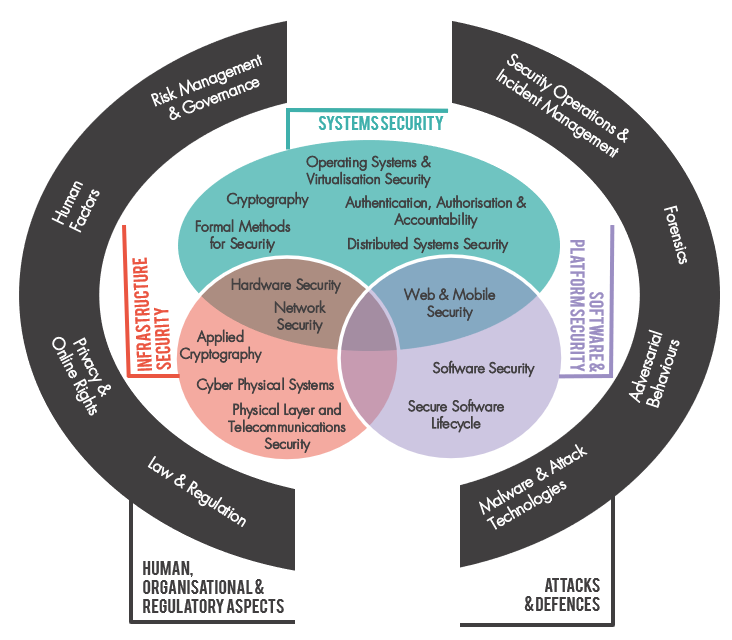
\includegraphics[keepaspectratio]{content/images/clipboard-695334883.png}}

}

\caption{Graphic showing the CyBOK KAs
(\href{https://www.cybok.org/media/article_images/2021/07/21/cybok_v_1_1.png}{source})}

\end{figure}%

CyBOK enables work to happen that would otherwise be very difficult. It
provides, for instance, a framework for assessing and communicating the
content of cyber security degree programmes, or for mapping out the
research profiles of cyber security scholars within a university. It
provides a common terminology for making comparisons and building up
composite profiles.

The UKCSC created its own classification system of 15 specialisms. Where
CyBOK focuses on `knowledge areas', the UKCSC specialisms are intended
to map onto types of cyber security job role. Each knowledge area may be
relevant to many specialisms, and each specialism may require several
knowledge areas. As part of its cyber careers framework, the UKCSC
provided a mapping of CyBOK to the specialisms, using four levels of
relevance (`core', `related', `wider' and non-relevant). Security
Operations \& Incident Management is the most well represented knowledge
area within the UKCSC Careers Framework, core to 6 specialisms, followed
by Law \& Regulation, which is core to 4 specialisms. Three knowledge
areas are not `core' for any specialisms: Human Factors, Operating
Systems and Virtualisation Security, and Physical Layer and Telecoms
Security\footnote{Formal Methods and Applied Cryptography are not
  included due to being added in the 2021 CyBOK 1.1 update.}. Quite
what, if anything, one should read into this is unclear: are these areas
that are deemed less `in demand' by industry? Or are they considered too
specialist for the kind of typology that the Careers Framework is
bringing together?

All classification systems have downsides. One downside is the
propensity to create path dependencies. Classification systems are a
kind of \emph{knowledge infrastructure}, and like all infrastructure,
once other systems come to depend on them, the costs of changing things
later on can be high, leading to slow, incremental change and incentives
against radical redesign. We encountered this challenge in our research.
Our effort to expand the scope of our analysis by adding 5 new
categories alongside the standard CyBOK KAs created challenges: because
only the original KAs are mapped to the UKCSC specialisms, we could not
incorporate new categories in our alignment calculations. Established
classifications in this way condition which questions are easier and
which are harder to answer.

Another downside is the fact that in prioritising some differences as
the basis of their scheme, classification systems make other differences
less visible. This can lead to `blindspots' (to take the metaphor
seriously, a blindspot is more than a gap in the visual field, it is a
gap that cannot easily be perceived\footnote{Try
  \url{https://www.scientificamerican.com/article/find-your-blind-spot/}}).
CyBOK was developed through a collaborative process that aimed to
capture established knowledge areas in cyber security. While this
process recognised the relevance of the social sciences to cyber
security, much of the diversity of social scientific knowledge was
bundled into the `human factors' category. The differences in
explanatory approaches across psychology, sociology, economics,
organisation studies, design and anthropology therefore become harder to
see. Social scientific expertise becomes invisible in the UKCSC Careers
Framework, since human factors here are treated as `soft skills'. What
was initially marginal is thus made increasingly invisible as
classifications develop on top of each other.

\section{Data analysis}\label{data-analysis-1}

\subsection{Personal expertise within and beyond
CyBOK}\label{sec-personal-expertise-within-and-beyond-cybok}

When we asked respondents to rate their expertise and the expertise
required for problem scenarios, we gave them 5 additional categories
beyond those that are included in CyBOK 1.1 (Martin et al. 2021). We
developed these based on discussions during the survey design process
with stakeholders from government and industry, and we selected 5 to
address:

\begin{itemize}
\item
  Areas that are growing in prominence, since CyBOK was first devised,
  and likely to continue growing. We thus included \emph{Data Science/AI
  for cyber security}. AI has been considered through a CyBOK `topic
  guide' and `knowledge guide', but as yet does not have the status of a
  knowledge area.
\item
  An area that is well established but happened to be left out from
  CyBOK. \emph{Cloud Security} was excluded from consideration within
  the Network Security knowledge area. Related considerations are
  included within Operating System and Virtualisation Security, but the
  lack of prominence within CyBOK is notably at odds with the importance
  of cloud security expertise in industry.
\item
  Creating more space for sociotechnical cyber security expertise.
  CyBOK's Human Factors knowledge area includes considerations of
  `positive security', but `human factors' is an inherently technology
  centric frame, referring to the `fit' between the human and the
  machine (Meister 2018). It is conceptually a poor home for expertise
  based in the recognition that security may be, primarily, a matter of
  value and values. Security culture and security awareness, other areas
  of expertise that draw on ideas and methodologies from the humanities
  and social sciences, straddle Human Factors and Risk Management and
  Governance knowledge areas. To explore sociotechnical dimensions more
  fully, we experimented with the inclusion of:

  \begin{itemize}
  \item
    \emph{Social organisational, strategy and process}
  \item
    \emph{Security culture, narrative and communication}
  \item
    \emph{Political aspects of cyber security}
  \end{itemize}
\end{itemize}

The addition of these five categories is not intended to `complete'
CyBOK, but to explore what we miss from the analysis when we rely on
standardised ways of dividing up the world. In
Figure~\ref{fig-personal-comb-overall} and
Figure~\ref{fig-scenario-comb-overall}, \emph{Data Science and AI for
Cyber Security} was relatively low in prominence within respondents'
answers for personal and scenario combs. Understanding how areas like
this may be gaining in prominence, and when they have crossed an
appropriate threshold for consideration within the Careers Framework,
will require that data collection steps outside of the standard
categories. The other four areas, on the other hand, were widely
recognised as elements of respondents' expertise. However, while many
respondents considered themselves relatively expert in \emph{Political
Aspects of Cyber Security} it is unlikely that this expertise is based
in substantial understanding of political theory or political
philosophy. It is a further challenge for the recognition of
sociotechnical expertise in cyber security that such expertise is
loosely defined.

The figure below shows on the x axis each respondent's maximum alignment
score, plotted against (on the y axis) the fraction of their comb that
is covered by CyBOK. There is no significant correlation gives us
confidence that the inclusion of our additional categories was not
significantly skewing the personal alignment metric results.

\begin{figure}

\centering{

\pandocbounded{
\includegraphics[keepaspectratio]{content/diversity_files/figure-pdf/fig-personal-CyBOKvsalignment-1.pdf}}

}

\caption{\label{fig-personal-CyBOKvsalignment}Percentage of expertise
comb covered by CyBOK, versus maximum specialism alignment}

\end{figure}%

The same cannot be said for the scenario alignment calculations. In some
cases, the 5 additional categories featured prominently in the expertise
required, and in these cases it is hard to say whether the UKCSC
specialisms are aligned. We comment on this below.

\subsection{Participants' comments on
classifications}\label{participants-comments-on-classifications}

The challenges of recognising and using classifications were visible to
survey participants, and several comments questions whether the
categories being used were appropriate:

\begin{tcolorbox}[enhanced jigsaw, leftrule=.75mm, colframe=quarto-callout-note-color-frame, opacityback=0, breakable, left=2mm, rightrule=.15mm, bottomrule=.15mm, colback=white, arc=.35mm, toprule=.15mm]

``The categories aren't what I was expecting. For example, why would web
be in the same category as mobile?''

\end{tcolorbox}

\begin{tcolorbox}[enhanced jigsaw, leftrule=.75mm, colframe=quarto-callout-note-color-frame, opacityback=0, breakable, left=2mm, rightrule=.15mm, bottomrule=.15mm, colback=white, arc=.35mm, toprule=.15mm]

``It felt like I was looking at one of a number of potential `combs',
i.e.~I have skills and knowledge that I have used throughout my career
that is not represented in the CyBOK.''

\end{tcolorbox}

One would always expect a certain amount of friction when presenting
people with classifications that reduce complexity into standard
categories. However, one should also be attentive to the
classification's alignment with the field. Further research into
expertise diversity in cyber security could generate input into CyBOK to
help the framework address gaps and to adapt to the changing landscape
of cyber security expertise and technology.

\subsection{The value of social and human
expertise}\label{the-value-of-social-and-human-expertise}

\begin{tcolorbox}[enhanced jigsaw, leftrule=.75mm, colframe=quarto-callout-note-color-frame, opacityback=0, breakable, left=2mm, rightrule=.15mm, bottomrule=.15mm, colback=white, arc=.35mm, toprule=.15mm]

``{[}The profession is{]} Not diverse enough. Cognitively.

Part of this is a function of who naturally gravitates towards the area.
Some of it is nurtured by ``professionalisation'', and coteries of
certification cabals. Institutionalises a mind set. Exact opposite of
what we need.

Best people I ever recruited had humanities backgrounds (archeology or
Anglo Saxon English); because they had critical thinking, communication
skills and a desire to learn.''

\end{tcolorbox}

Some degree of familiarity in human communication, behaviour, critical
analysis and social explanation is picked up `on the job', but having
good `soft skills' is entirely different from being competent in the
sciences of communication, behaviour, politics and society. We do not
confuse being a mathematician with general numeracy: when you train as a
mathematician you do not simply become very numerate (indeed many fields
of mathematics are not about numbers at all). When you train as a
mathematician you learn a family of techniques and a body of knowledge.
Clarifying this distinction and why it matters for cyber security should
be a priority for sociotechnical security research.

\begin{tcolorbox}[enhanced jigsaw, leftrule=.75mm, colframe=quarto-callout-note-color-frame, opacityback=0, breakable, left=2mm, rightrule=.15mm, bottomrule=.15mm, colback=white, arc=.35mm, toprule=.15mm]

``I think the cybersecurity profession focuses too much on technical
security skills and not enough on transferable soft skills. We would not
have such a diversity and recruitment problem in security, if we could
embrace those skills like being able to manage a project, communicate
with a board or problem solve. These are experiences gained in a wide
range of job roles. We should value that expertise as much as the
technical security skills, as without the ability to influence,
communicate, change something or solve a problem, how can we drive any
improvement.''

\end{tcolorbox}

\begin{tcolorbox}[enhanced jigsaw, leftrule=.75mm, colframe=quarto-callout-note-color-frame, opacityback=0, breakable, left=2mm, rightrule=.15mm, bottomrule=.15mm, colback=white, arc=.35mm, toprule=.15mm]

``we have an image problem in cybersecurity - we think the cool image is
of a hoody wearing hacker in front of a keyboard / laptop, whether they
are good guys or bad guys. The problem is this means we do not encourage
the broader roles of cyber that are so not about the technology or the
pen testing or hacking skills.

My concern with the chartered status efforts the easy route will be to
focus on chartering the technology centric aspects and roles and thus
alienate those sitting on the outskirts of the tech often driving
forward change and leading major cyber security efforts.''

\end{tcolorbox}

Respondents' concerns with the overplayed `technology centric' aspects
of cyber security raises a broader issue with the technology and EDI
agenda. The goal of increasing the representation of women in technology
jobs has motivated campaigns to draw more women into STEM subjects in
further and higher education. There is no doubt that this has been
highly valuable. But there is an additional narrative that is implied
here that is not necessarily helpful: that social scientific and
humanities skills are not relevant to technology jobs. Changing the
narrative to emphasise the contribution of the social sciences and
humanities within tech and within cyber security may be needed,
especially as AI technologies change skillsets. To do this effectively
it will be necessary to see better representation of these forms of
expertise in professional classifications.

\section{Recommendations}\label{recommendations-2}

Future iterations of the Cybersecurity Body of Knowledge (CyBOK) should
be informed by research into expertise diversity, to ensure that the
value of the humanities and social sciences within cyber security is
better reflected.

\bookmarksetup{startatroot}

\chapter{Interdisciplinarity}\label{interdisciplinarity}

\section{Interdisciplinary cyber
security}\label{interdisciplinary-cyber-security}

In this section we were interested in how one might analyse the
interdisciplinary of cyber security practice. Understanding the value of
diversity of expertise in cyber security requires a view of the problems
that arise in cyber security, and the kinds of combinations of expertise
that they require. For organisations, the utility of professional
classifications depends on the extent to which it is possible to
identify a need for particular kinds of expertise. Understanding the
alignment of specialisms with scenarios that are representative of
organisations' practical cyber security problems is one way to approach
this. The Cyber Expertise Diversity Survey elicited such profiles from
respondents, for a range of scenarios. Qualitative descriptions of these
scenarios help us to explore the ways in which scenarios map onto
specialisms, in particular:

\begin{itemize}
\item
  Which scenarios map straightforwardly onto one specialism
\item
  Which scenarios require combinations of specialisms
\item
  Which scenarios require significant expertise that is not accounted
  for by the specialisms
\end{itemize}

\section{Data analysis}\label{data-analysis-2}

\subsection{Respondents and scenarios}\label{respondents-and-scenarios}

\begin{figure*}

\centering{

\pandocbounded{
\includegraphics[keepaspectratio]{content/interdisciplinarity_files/figure-pdf/fig-alignment-persona-vs-scenarios-1.pdf}}

}

\caption{\label{fig-alignment-persona-vs-scenarios}Personal vs Scenarios
alignment}

\end{figure*}%

This graph plots the difference between the personal alignment metric
and scenario alignment metric for each individual respondent. Each line
shows the difference between these two responses. Purple shows those
responses where personal skills exceed those needed for the scenario
described. Teal shows those where the skills needed for the scenario
exceed those of the respondent. At a very high level this gives a sense
of the breadth and depth of the profession as represented in our sample.

\subsection{Looking at specialisms alignment with the
scenarios}\label{looking-at-specialisms-alignment-with-the-scenarios}

\subsubsection{Alignment of permutations of multiple specialisms with
problem
scenarios}\label{alignment-of-permutations-of-multiple-specialisms-with-problem-scenarios}

We calculated the alignment of the UKCSC specialisms with the scenarios
our respondents told us about. We were interested in how alignment
scores would increase if we allowed permutations of two or more
specialisms. Figure~\ref{fig-alignment-scenarios-overview} shows that,
on average, the alignment index increases as we increase the number of
permutations (this is, these scenarios are more interdisciplinary).
While this could be expected, this is not the case for every scenario,
as shown in Figure~\ref{fig-alignment-scenarios}, which provides a more
nuanced view by displaying how the alignment score changes for every
scenario.

\begin{figure}

\centering{

\pandocbounded{
\includegraphics[keepaspectratio]{content/interdisciplinarity_files/figure-pdf/fig-alignment-scenarios-overview-1.pdf}}

}

\caption{\label{fig-alignment-scenarios-overview}Alignment indices per
number of permutations}

\end{figure}%

In the graphs below, a steep gradient indicates significantly better
alignment could be gained through mixed teams of specialists. The
alignment score for permutations of specialists is calculated by
creating combined `combs'. We do this for all possible permutations, up
to a maximum of 5, and plot how the maximum alignment for each scenario
increases. The sliders for 25, 31, 44 and 53 were left blank, but we
include for completeness.

\begin{figure*}

\centering{

\pandocbounded{
\includegraphics[keepaspectratio]{content/interdisciplinarity_files/figure-pdf/fig-alignment-scenarios-1.pdf}}

}

\caption{\label{fig-alignment-scenarios}Alignment indices per number of
permutations and scenario}

\end{figure*}%

\subsection{Discussion}\label{discussion}

\subsubsection{Lowest alignment
scenarios}\label{lowest-alignment-scenarios}

Scenarios that have lower overall alignment tend to be scenarios where
respondents set the combs particularly `full'. For instance, for
\emph{Scenario 3: global mass use of malware}, the participant set all
sliders to 100 (or nearly). \emph{Scenario 13: investigation of a cyber
incident}: apart from a few (data science, hardware, cyber physical and
cryptography), this was deemed to require a very `full' comb. Similarly,
\emph{Scenario 28: Develop effective and real world governance to
protect assets while facilitating and enabling business goals and
objectives} had a very `full' comb.

\subsubsection{Most interdisciplinary
scenarios}\label{most-interdisciplinary-scenarios}

Scenarios that had a steep gradient may be interpreted as particularly
interdisciplinary. The adequacy of a team to tackle these scenarios
improves significantly if more different specialists are added.
\emph{Scenario 7: Protecting Legacy equipment against emerging AI/PQC
Threat}, for instance combined significant elements of `hardware
security', `cryptography', `network security', `authentication,
authorisation and accountability', and `distributed systems security'.
Scenarios like this hit a combination of expertise that is not directly
associated within existing specialisms. No UKCSC specialism, for
instance, is identified with `authentication, authorisation and
accountability' \emph{and} `hardware security'. This scenario is about
protecting legacy equipment in a CNI context, widely understood to be a
key problem area in the profession. In this case the best alignment was
achieved as follows:

1 Specialist: Secure System Architecture \& Design (Industrial Control
Systems)

2 Specialists: Incident response (Industrial Control Systems),
Cryptography \& Communications Security (Cryptographer)

3 Specialists: Cyber Threat Intelligence, Cryptography \& Communications
Security (Cryptographer), Secure System Architecture \& Design
(Industrial Control Systems)

4 Specialists: Cyber Threat Intelligence, Cryptography \& Communications
Security (Cryptographer), Secure Operations, Secure System Architecture
\& Design (Industrial Control Systems)''

5 Specialists: Cyber Threat Intelligence, Cyber Security Management,
Cryptography \& Communications Security (Cryptographer), Secure
Operations, Secure System Architecture \& Design (Industrial Control
Systems)''

Scenario 27: incident response was intriguing. It was also very
`interdisciplinarity' looking at the gradient that we are using for a
heuristic. But this is puzzling because there is a specialism called
`incident response' that one might presume ought to align well on its
own. The respondent had specified the problem scenario including the
requirement for very high expertise in `authorisation, authentication
and accountability', and quite high in `operating systems and
virtualization security'. Neither of these are taken to be of even
`wider' relevance to incident response. Indeed, the incident response
specialism did not feature in any of the best combinations of
specialisms for this scenario. While this is highly anecdotal, it does
suggest there is more to be understood, and that there could be
improvements to the Cyber Careers Framework's CyBOK mapping to ensure
good alignment with practice.

Scenarios 61 and 62 were more specialist problems

\begin{tcolorbox}[enhanced jigsaw, leftrule=.75mm, colframe=quarto-callout-note-color-frame, opacityback=0, breakable, left=2mm, rightrule=.15mm, bottomrule=.15mm, colback=white, arc=.35mm, toprule=.15mm]

Got pulled from a job testing building management/HVAC systems to taking
lead on assessing encrypted VoIP systems. Had to give a crash course on
OT testing to more junior colleagues before switching assignments (61)

\end{tcolorbox}

Scenario 61 involved a wide spread of expertise, while scenario 62
required high expertise in a relatively high number of areas.

\begin{tcolorbox}[enhanced jigsaw, leftrule=.75mm, colframe=quarto-callout-note-color-frame, opacityback=0, breakable, left=2mm, rightrule=.15mm, bottomrule=.15mm, colback=white, arc=.35mm, toprule=.15mm]

Requirement to build out a cyclical, threat detection and engineering
process which required:

\begin{itemize}
\item
  Understanding of Primary Threat Adversaries and identification of
  their TTPs.
\item
  Threat Hunting capability for aforementioned TTPs (and other
  Indicators of Compromise).
\item
  Detection Engineering capability (for creation of signals, signatures
  and detections, specific to the aforementioned TTPs), delivering these
  into production.
\item
  Event Triage and Investigation to Incident esclation including
  containment, eradication and recovery.
\item
  Feedback mechansim of observed incidents, back into Intelligence teams
  to close the loop. (Detection Lifecycle Management).

  (62)
\end{itemize}

\end{tcolorbox}

These scenarios are the more `naturally' interdisciplinary cases, where
problems need to be addressed that are idiosyncratic, are not neatly
contained within standard specialism areas, and will either require
individuals with unusual skillsets or else mixed teams.

\subsubsection{Non-CyBOK expertise}\label{non-cybok-expertise}

Finally, some scenarios were specified in ways that heavily emphasised
the need for non-CyBOK areas of expertise. In these cases, the alignment
scores are deceptive, because we cannot calculate which specialists
would contribute these skills. Interestingly, one of these cases was
\emph{58 - Incident Response is a business requirement, not just for the
IT/Cyber team(s).}

\begin{tcolorbox}[enhanced jigsaw, leftrule=.75mm, colframe=quarto-callout-note-color-frame, opacityback=0, breakable, left=2mm, rightrule=.15mm, bottomrule=.15mm, colback=white, arc=.35mm, toprule=.15mm]

Often people think that cyber maturity, resilience, and response is just
for the cyber or IT teams to do. Promoting that it there are multiple
groups that will be affected and impacted by a successful compromise and
making them aware and appreciate their role to play and to consider what
their individual playbook would look like is a difficult but important
task to achieve. Evidence based metrics to promote the risk and then
cyber resilience exercises involving key stakeholders that then promote
wider engagement down the line is a necessary tool to have in your
armour. (58)

\end{tcolorbox}

Incident response is supposed to be captured within the existing
specialisms, but this respondent specifies the problem in a way that
emphasises expertise that is not considered within the Careers
Framework. In particular, the organisational, human factors and culture
aspects are deemed particularly important. Again anecdotal, examples
like this are suggestive that these areas are perhaps more diverse in
their needs, or in the approaches that practitioners take, than is
usually recognised. Given that several respondents voiced scepticism
about the value of certifications, ensuring alignment of the specialisms
with real world problems is likely to be crucial to long term success.
This means examining the adequacy of the current framework, examining
how problems are changing with new technology and new threats, and
examining problem definition more broadly.

\section{Recommendations}\label{recommendations-3}

The UK Cyber Security Council's Cyber Career Framework's cross-reference
to CyBOK should be refined and validated through studies of cyber
security problem scenarios.

\bookmarksetup{startatroot}

\chapter{Conclusions}\label{conclusions}

`More research is needed' is never a satisfying conclusion to draw, but
in a rapidly evolving sector these kinds of conclusions are crucial in
ensuring that future research lines up with key questions.

\begin{itemize}
\item
  We need data that helps us to establish relationships between
  diversity and expertise, to influence the process of
  professionalisation. We have argued that this evidence base would be a
  key enabler for the credibility of professional categories, and
  ultimately for strengthening the UK's cyber security capacity. We have
  argued that future Decrypting Diversity studies would be of great
  value to the profession especially if they incorporate attention to
  expertise in the way we have prototyped here.
\item
  This data can help inform classifications such as CyBOK and the Cyber
  Careers Framework, ensure that gaps are filled and the profession is
  responsive to new areas of expertise as it adapts to changing
  technological and social circumstances.
\item
  In parallel with seeking to build the evidence base, we feel it would
  be worthwhile for exploratory work to be undertaken to map out what
  new specialisms in areas such as security human factors and security
  awareness could look like. This would be valuable because once they
  are scoped out, the alignment of these specialisms with cyber security
  scenarios could be tested through data analysis.
\item
  We were unable to develop a detailed analysis of the value of
  idiosyncratic career pathways to cyber security but this remains an
  issue worthy of further investigation, given that professionalisation
  is likely to guide the careers of future professionals along
  increasingly conventionalised pathways.
\item
  We have sought to contextualise this work within bodies of literature
  on professionalisation, classification and diversity, which we hope
  will help to provide strong theoretical foundations for future
  analyses.
\end{itemize}

We would like to thank all our respondents for the time they gave us in
filling in the survey, and to the generous individuals from industry and
government who helped us to define the project.

\bookmarksetup{startatroot}

\chapter*{References}\label{references}
\addcontentsline{toc}{chapter}{References}

\markboth{References}{References}

\phantomsection\label{refs}
\begin{CSLReferences}{1}{0}
\bibitem[\citeproctext]{ref-attwood2023exploring}
Attwood, Sam, and Ashley Williams. 2023. {``Exploring the UK Cyber
Skills Gap Through a Mapping of Active Job Listings to the Cyber
Security Body of Knowledge (CyBOK).''} In \emph{Proceedings of the 27th
International Conference on Evaluation and Assessment in Software
Engineering}, 273--78.

\bibitem[\citeproctext]{ref-bowker1999sorting}
Bowker, Geoffrey, and Susan Leigh Star. 1999. {``Sorting Things Out.''}
\emph{Classification and Its Consequences} 4.

\bibitem[\citeproctext]{ref-cabinetofficeGovernmentCyberSecurity2022}
Cabinet Office, ed. 2022. {``Government {Cyber Security Strategy}: 2022
to 2030.''}
\url{https://assets.publishing.service.gov.uk/media/61f0169de90e070375c230a8/government-cyber-security-strategy.pdf}.

\bibitem[\citeproctext]{ref-Camara-Menoyo_The_Cyber_Expertise_2025}
Cámara-Menoyo, Carlos, Matt Spencer, and Timothy Monteath. 2025. {``The
{Cyber Expertise Diversity Survey Dataset}.''}
https://github.com/WarwickCIM/cyberexpertisediversity\_survey\_data.
\url{https://doi.org/10.17605/OSF.IO/GX7ME}.

\bibitem[\citeproctext]{ref-daniel2007outsiders}
Daniel, CarolAnn. 2007. {``Outsiders-Within: Critical Race Theory,
Graduate Education and Barriers to Professionalization.''} \emph{J. Soc.
\& Soc. Welfare} 34: 25.

\bibitem[\citeproctext]{ref-dekker2014drifting}
Dekker, Sidney, and Shawn Pruchnicki. 2014. {``Drifting into Failure:
Theorising the Dynamics of Disaster Incubation.''} \emph{Theoretical
Issues in Ergonomics Science} 15 (6): 534--44.

\bibitem[\citeproctext]{ref-evetts2012similarities}
Evetts, Julia. 2012. {``Similarities in Contexts and Theorizing:
Professionalism and Inequality.''} \emph{Professions and
Professionalism} 2 (2).

\bibitem[\citeproctext]{ref-grabher1997organizing}
Grabher, Gernot, and David Stark. 1997. {``Organizing Diversity:
Evolutionary Theory, Network Analysis and Postsocialism.''}
\emph{Regional Studies} 31 (5): 533--44.

\bibitem[\citeproctext]{ref-herring2009does}
Herring, Cedric. 2009. {``Does Diversity Pay?: Race, Gender, and the
Business Case for Diversity.''} \emph{American Sociological Review} 74
(2): 208--24.

\bibitem[\citeproctext]{ref-levine2014ethnic}
Levine, Sheen S, Evan P Apfelbaum, Mark Bernard, Valerie L Bartelt,
Edward J Zajac, and David Stark. 2014. {``Ethnic Diversity Deflates
Price Bubbles.''} \emph{Proceedings of the National Academy of Sciences}
111 (52): 18524--29.

\bibitem[\citeproctext]{ref-cybok}
Martin, Andrew, Awais Rashid, Howard Chivers, George Danezis, Steve
Schneider, and Emil Lupu. 2021. \emph{The Cyber Security Body of
Knowledge}. 1.1 ed. University of Bristol. \url{https://www.cybok.org/}.

\bibitem[\citeproctext]{ref-meister2018history}
Meister, David. 2018. \emph{The History of Human Factors and
Ergonomics}. CRC Press.

\bibitem[\citeproctext]{ref-DefenceSecurityIndustrial2021}
Ministry of Defence, ed. 2021. \emph{Defence and {Security Industrial
Strategy}: {A} Strategic Approach to the {UK}'s Defence and Security
Industrial Sectors}. London: Dandy Booksellers Ltd.
\url{https://assets.publishing.service.gov.uk/media/60590e988fa8f545d879f0aa/Defence_and_Security_Industrial_Strategy_-_FINAL.pdf}.

\bibitem[\citeproctext]{ref-nationalcybersecuritycentreDecryptingDiversityDiversity2021}
National Cyber Security Centre. 2021. {``Decrypting Diversity:
{Diversity} and Inclusion in Cyber Security Report 2021.''}
\url{https://www.ncsc.gov.uk/report/decrypting-diversity-2021-diversity-and-inclusion-in-cyber-security}.

\bibitem[\citeproctext]{ref-nautiyal2024framework}
Nautiyal, Lata, and Awais Rashid. 2024. {``A Framework for Mapping
Organisational Workforce Knowledge Profile in Cyber Security.''}
\emph{Computers \& Security} 145: 103925.

\bibitem[\citeproctext]{ref-NCSC2020decrypting}
NCSC, KPMG. 2020. {``Decrypting Diversity: Diversity and Inclusion in
Cyber Security.''} National Cyber Security Centre.

\bibitem[\citeproctext]{ref-vaughan1996challenger}
Vaughan, Diane. 1996. \emph{The Challenger Launch Decision: Risky
Technology, Culture, and Deviance at NASA}. University of Chicago press.

\bibitem[\citeproctext]{ref-weber2019economy}
Weber, Max. 2019. \emph{Economy and Society: A New Translation}. Harvard
University Press.

\bibitem[\citeproctext]{ref-weick1987organizational}
Weick, Karl E. 1987. {``Organizational Culture as a Source of High
Reliability.''} \emph{California Management Review} 29 (2): 112--27.

\bibitem[\citeproctext]{ref-wilkinson2016}
Wilkinson, Mark D., Michel Dumontier, IJsbrand Jan Aalbersberg,
Gabrielle Appleton, Myles Axton, Arie Baak, Niklas Blomberg, et al.
2016. {``The FAIR Guiding Principles for Scientific Data Management and
Stewardship.''} \emph{Scientific Data} 3 (1): 160018.
\url{https://doi.org/10.1038/sdata.2016.18}.

\end{CSLReferences}


\backmatter


\end{document}
